%\documentclass[conference]{IEEEtran}

\documentclass[12pt,onecolumn]{article}

%\documentclass[journal,draftclsnofoot,12pt,onecolumn]{IEEEtran}

\usepackage{cite}
\usepackage{color}
\usepackage{amsmath}
\usepackage{graphicx}

\usepackage{algorithm}
\usepackage{algorithmic}

\usepackage[table]{xcolor}

\definecolor{light-gray}{gray}{0.95}

% correct bad hyphenation here
\hyphenation{wire-less net-works}

\begin{document}

\title{\textbf{Long-Term Evolution in Unlicensed Bands: Current Status and Potential Research Directions}}

%\author{
%\IEEEauthorblockN{Quang-Dung Ho, Daniel Tweed, and Tho Le-Ngoc}\\
%\IEEEauthorblockA{Department of Electrical and Computer Engineering\\
%McGill University, Montreal, Quebec, Canada}}

\author{Quang-Dung Ho, Daniel Tweed, and Tho Le-Ngoc\\
\\\vspace{6pt} Department of Electrical and Computer Engineering\\
McGill University, Montreal, Quebec, Canada}


\maketitle


\begin{abstract}


\textsf{Global mobile traffic is expected to increase nearly tenfold between 2014 and 2019 due to increasing number of mobile-connected devices and the explosion of data-hungry mobile applications \cite{cisco_mobile_traffic_2015}. Pushing traffic towards the network capacity quickly deteriorates the Quality of Services (QoSs) perceived by the users. Acquiring additional licensed spectrum to increase the capacity of Radio Access Networks (RANs) is certainly very expensive. Mobile operators are also challenged by the ``revenue gap'', i.e., the exponential increase in mobile traffic does not generate sufficient additional revenues required for upgrading their RANs. This circumstance has fostered the interest in cost-effective solutions to increase the capacity of RANs. Long-Term Evolution (LTE) in unlicensed bands (U-LTE) is among promising solutions. However, since U-LTE is a nascent LTE technology, there are still various associated concerns and challenges to be addressed.}

\textsf{This work \textit{first} presents a comprehensive survey on U-LTE, focusing on various mechanisms used for the coexistence of this technology and others in shared frequency bands. Specifically, for background knowledge, concepts, motivations, benefits, and obstacles of U-LTE are presented. Three typical types of U-LTE including LTE-U, LAA-LTE, and MuLTEfire are explained. Next, regulations specified by standard institutes for radio systems operating in unlicensed spectrum are reviewed. Additionally, due to the fact that in-depth knowledge on IEEE 802.11/Wi-Fi CSMA-CA protocol is strongly required to understand and analyze the interactions between U-LTE and Wi-Fi when they operate in the same frequency band, details of CSMA-CA protocol as well as its distinguishing features compared to standardized regulations are presented. \textit{Second}, in order to capture the ongoing activities on U-LTE's coexistence mechanisms, related works are surveyed with insight observations on their limitations and concerns. \textit{Finally}, towards future working directions, in the light of the survey this work identifies a number of open technical questions as well as related potential research issues in U-LTE.}

\end{abstract}

%\IEEEpeerreviewmaketitle


%**************************************************************************************************************%
\tableofcontents

\listoffigures




%**************************************************************************************************************%

\section{Introduction}
\label{sec:introduction}

\subsection{Motivation and Concept of U-LTE}

\noindent U-LTE is a promising approach to address the revenue gap in mobile communications networks. By definition, it is an LTE technology that puts cellular signals into the unlicensed spectrum with the supports of existing LTE features including Supplemental Downlink (SDL, proposed in LTE Release 9 and later) and Carrier Aggregation (CA, proposed in LTE Release 10 and later). The original idea of LTE-U is fairly straightforward. As mentioned, mobile operators are facing a great pressure on capacity and cost. If LTE can exploit the unlicensed band (where IEEE 802.11/Wi-Fi and other radio systems are using), then it will have a considerable additional capacity at a minimal cost. U-LTE can be used to boost downlink or both uplink and downlink of LTE networks, as illustrated in Fig. \ref{figs:U-LTE-use_model}.

U-LTE was first officially announced by Qualcomm in 2013 \cite{Qualcomm-U-LTE-2013}. Currently, it focuses on $500$ MHz of spectrum available in the $5$ GHz band. Specifically, according to the proposal from Qualcomm, U-LTE uses the U-NII-3 part of the $5$ GHz band, which has highest allowed Equivalent Isotropically Radiated Power (EIRP). While in $2.4$ GHz regulatory bodies limit EIRP to $100$ mW (in Europe) or $200$ mW (in United States), the U-NII-3 enjoys the rights to go as high as $1000$ mW outdoors.

\subsection{Benefits of U-LTE}

\noindent U-LTE is expected to offer numerous benefits to mobile network operators, service providers, and consumers. \textit{First}, free unlicensed spectrum provides additional capacity to the network at a minimal cost. Therefore, U-LTE appears to be a very inexpensive way to meet the future traffic growth. \textit{Second}, U-LTE will give operators the option to make use of unlicensed spectrum with a unified network, offering potential operational cost saving, improving spectral efficiency, and providing a better user experience. Compared to the Wi-Fi offloading technology, U-LTE has the potential to offer significantly better coverage and higher spectral efficiency while allowing seamless flow of data across licensed and unlicensed in a single core network. \textit{Third}, U-LTE could also take advantage of the robust security features of LTE networks. \textit{Finally}, while Wi-Fi offloading leads to less traffic on mobile networks and thus may result in revenue losses in data services, U-LTE could represent an incremental ability on mobile service providers to directly bill for data usage.

\begin{figure}[!t]
\centering
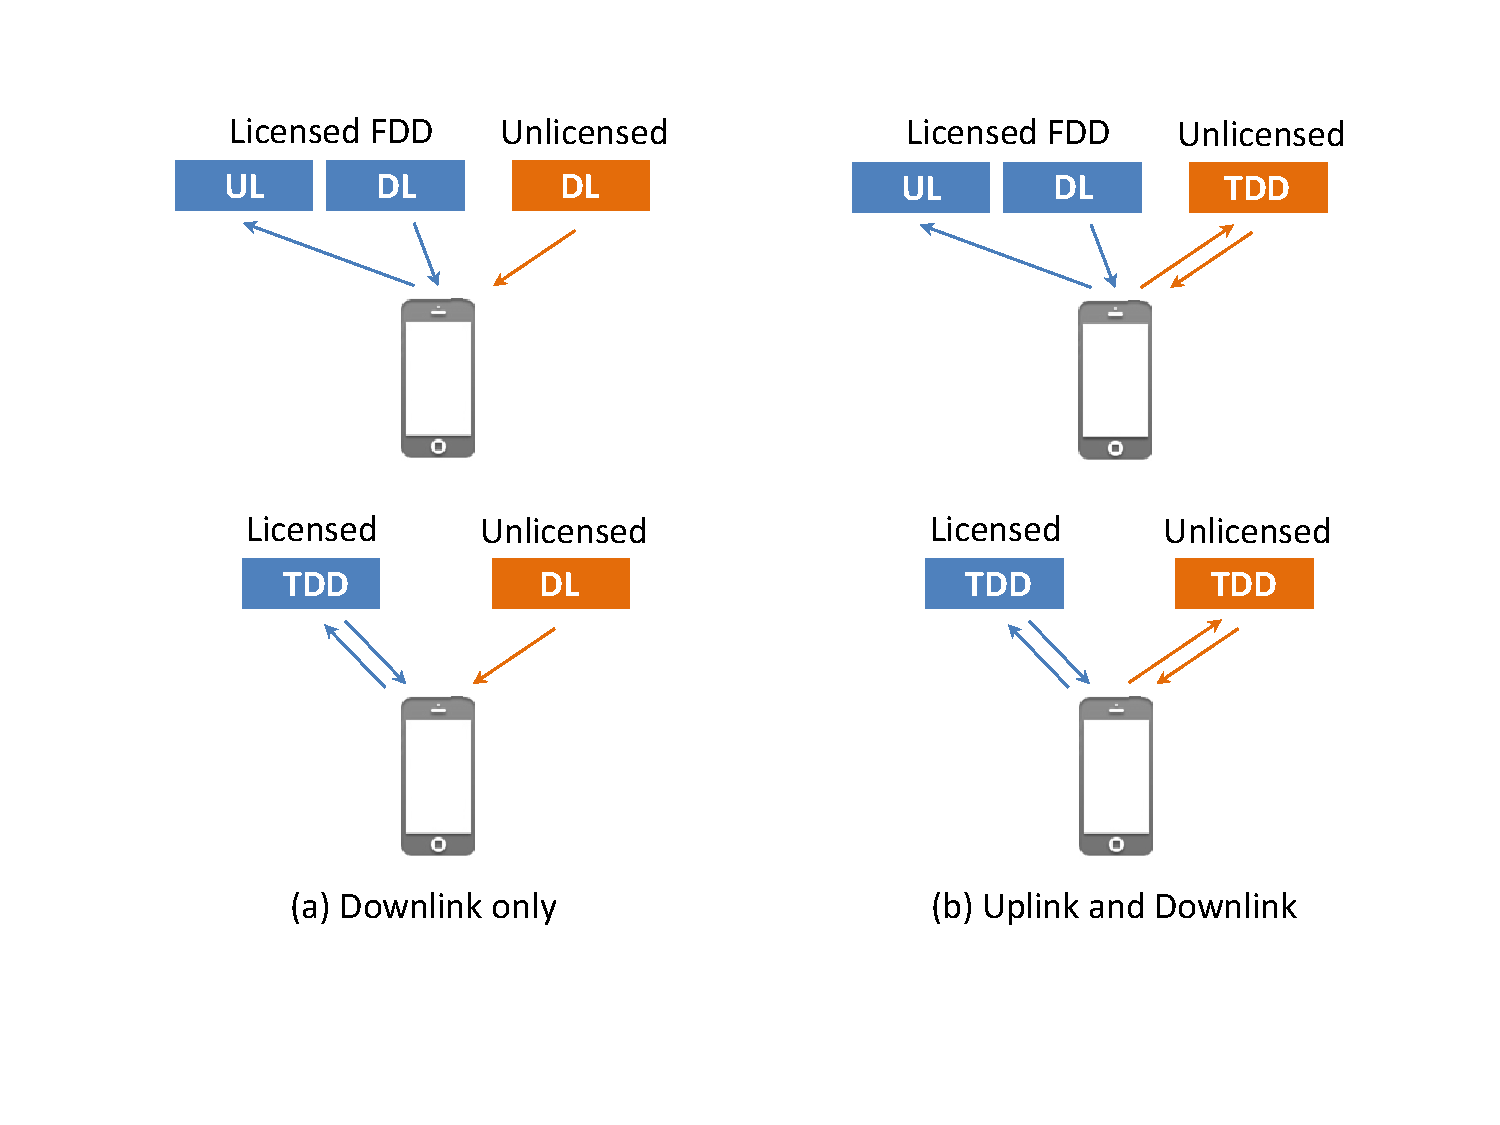
\includegraphics[width=0.7\columnwidth]{figures2/U-LTE-use_model}
\caption{Use cases of U-LTE.}
\label{figs:U-LTE-use_model}
\end{figure}

\subsection{Obstacles of U-LTE}

U-LTE is also facing a number of substantial obstacles. \textit{First}, even though U-LTE is not charged for the use of unlicensed spectrums, compared to Wi-Fi, its network deployment could be more expensive. LTE chipset itself is several times more expensive than that of Wi-Fi (a few tens of dollars compared to a few dollars or less than one dollar). LTE base stations and other network devices are likely to cost substantially more. Also, LTE operators need to deploy and maintain expensive back-haul links. \textit{Next}, U-LTE will work only with LTE-capable devices while there have been many more devices that feature Wi-Fi connectivity than LTE. Wi-Fi is nearly always integrated with laptops, tablets, cameras, and other connected consumer devices. \textit{Additionally}, from technical perspectives, the premium features provided by U-LTE (e.g., seamless voice and data roaming) may not prove sufficiently more valuable than those offered by emerging Wi-Fi technologies such as Hotspot 2.0, so-called Wi-Fi Certified Passpoint, which is a new standard for public-access Wi-Fi that enables seamless roaming among Wi-Fi networks and between Wi-Fi and cellular networks. \textit{Finally}, the biggest challenge of U-LTE is its coexistence with other radio networks operating in the same frequency bands. This challenge will be studied in subsequent sections. 

\subsection{Three Types of U-LTE}

\noindent U-LTE comprises of three different flavors: LTE unlicensed (LTE-U), Licensed Assisted Access LTE (LAA-LTE), and MuLTEfire. The first two flavors require ``anchoring licensed spectrum'', i.e., they operate primarily in licensed spectrum and opportunistically exploit unlicensed spectrum for an additional bandwidth boost. Devices are still anchored in licensed spectrum for LTE management/control signaling and high QoS data while using the unlicensed spectrum for only best-effort or delay-tolerant data. The third flavor is developed by Qualcomm and requires no licensed spectrum at all, therefore, it is often referred to as ``standalone'' U-LTE. MuLTEfire is designed for indoor use and deployments by enterprises, cable companies and other service providers without ownership of expensive bandwidth licenses. However, at present time, there are very few technical details available about MuLTEfire.

\subsection{Coexistence of U-LTE and Wi-Fi}

\noindent It is well known that multiple radio communications technologies operating in a common frequency band will negatively affect each other if respectful coexistence mechanisms are not employed. As a result, despite the fact that U-LTE can offer various benefits as mentioned before, its coexistence with Wi-Fi and other radio systems that operate in the $5$ GHz frequency band is the biggest concerns. In details, it has been believed that U-LTE may considerably interfere Wi-Fi systems and/or grasp more radio resources when they are operating in the same frequency band due to the following facts.

\textit{First}, LTE was originally designed to work in its own licensed band rather than to coexist with Wi-Fi in a shared band. LTE employs Orthogonal Frequency-Division Multiple Access (OFDMA) and transmits almost continuously without any mechanism for spectrum sharing. Wi-Fi, on the other hand, employs Listen Before Talk (LBT) MAC with a few key additional features that go beyond LBT requirements specified by European Telecommunications Standards Institute (ETSI) \cite{LBT-ETSI-2014}. As a result, U-LTE might overwhelm Wi-Fi neighbors with its aggressive transmissions if no relevant coexistence measure is implemented.

\textit{Second}, the typical lengths of each transmission of these two technologies are not the same. LTE, due to its basic protocol design and scheduled nature, generally transmits long frames (i.e., multiple ms), whereas a large percentage of Wi-Fi frames are sub-millisecond in duration. For this reason, equitable access to the medium, evaluated in terms of how often a technology is able to start a transmission, does not necessarily translate into equitable airtime.

\textit{Third}, a license-anchored system (LTE-U or LAA-LTE) operates simultaneously in licensed and unlicensed bands and thus can dynamically move traffic between the bands on a granular basis (e.g., per-user and per-flow). As a result, such a system is inherently less sensitive to collisions and congestion in the unlicensed bands than is a system operating solely in unlicensed spectrum. This may reduce the incentive for a license-anchored system to develop effective coexistence mechanisms in the unlicensed band.

In fact, U-LTE is still a nascent LTE technology with many technical details to be determined. Proponents of U-LTE include Qualcomm, Ericsson, Alcatel-Lucent, Huawei, LTE-U Forum, 3rd Generation Partnership Project (3GPP), Verizon Wireless, T-Mobile US, etc. At the same time, CableLabs, Google, Wi-Fi Alliance, The Institute of Electrical and Electronics Engineers Standards Association (IEEE-SA) and many Wi-Fi interested companies are participating in and following closely the development of U-LTE technology. They have been expressing their concern on a critical need for strong coexistence between U-LTE and Wi-Fi to ensure responsible and fair use of unlicensed spectrum. As a result, various studies on the coexistence of U-LTE and Wi-Fi have been carried out by both industry and academia. Besides, a number of reports and comments related to this concern have been filed with the Federal Communications Commission (FCC).

\subsection{Requirements of U-LTE Coexistence Mechanisms}

\noindent Even though the unlicensed bands may be used by anyone, there is a series of government guidelines and regulations to be followed. Those guidelines and regulations aim to ensure that different radio systems that operate in the same frequency bands are good neighbors of each other.

In particular, for coexistence with Wi-Fi, at least U-LTE must satisfy local regulations such as the maximum transmission power in specific bands and the avoidance of bands dedicated to protected services. Furthermore, an U-LTE system should not cause any higher interference to a neighboring Wi-Fi system than a typical Wi-Fi system operating on the same channel. In other words, the impact of a U-LTE device to Wi-Fi devices (in terms of collision rate and probability of successful channel access) should be similar to that caused by a typical Wi-Fi device. These requirements ask for inclusions of a number of new features in LTE. For example, U-LTE should select a carrier which is least occupied in the area and it should dynamically change operating frequency to avoid conflict with protected systems, such as radar. It should also apply LBT or Clear Channel Assessment (CCA) techniques to check that a channel is free before making a transmission. Exactly how these decisions are made will be key aspects of U-LTE system designs.

%**************************************************************************************************************%
\section{An Overview on ETSI's and Wi-Fi's LBT Mechanisms}
\label{sec:LBT-overview}

\subsection{ETSI's LBT Mechanisms}
\label{subsec:ETSI-LBT-overview}

In \cite{LBT-ETSI-2014}, ETSI describes a number of spectrum access requirements to facilitate spectrum sharing for wireless access systems in $5$ GHz frequency band. This subsections focuses on requirements related to LBT mechanisms by which an equipment or a device applies CCA before using the channel to avoid collisions. The first mechanism is Frame Based Equipment (FBE) which defines a fixed (not directly demand-driven) timing frame for channel access. The second mechanism is Load Based Equipment (LBE) which defines demand-driven timing frame.

\begin{figure}[!t]
\centering
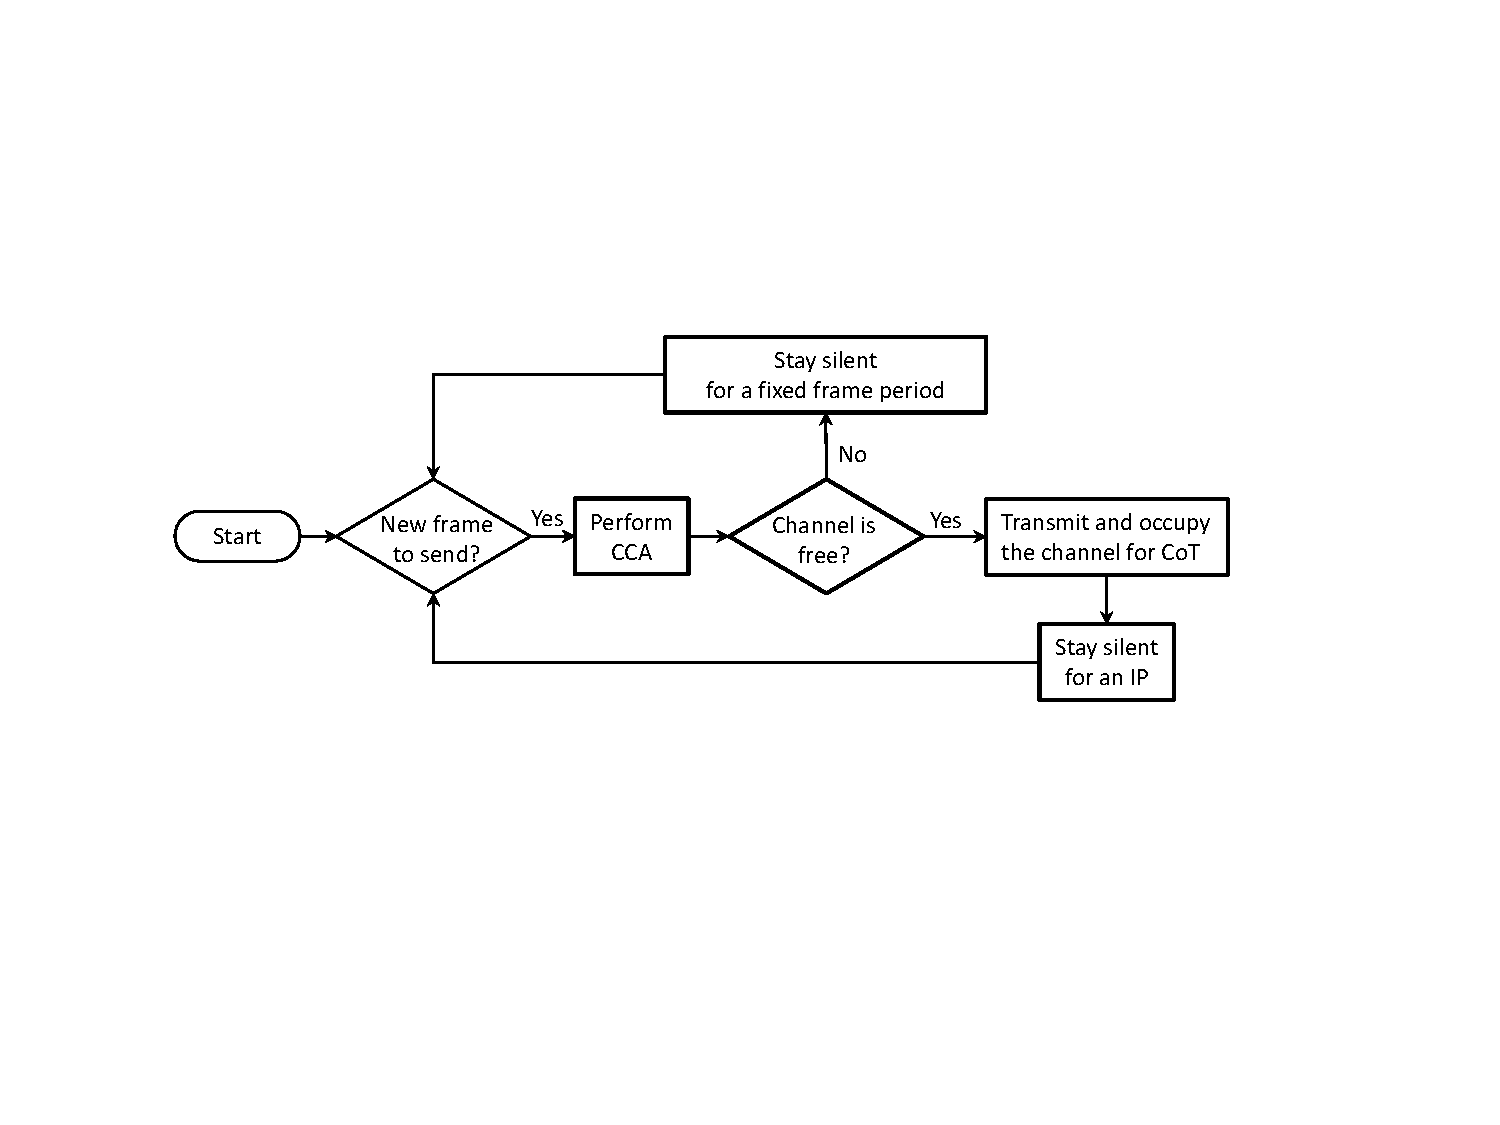
\includegraphics[width=0.9\columnwidth]{figures2/FBE-flowchart}
\caption{Simplified flowchart of FBE.}
\label{figs:FBE-flowchart}
\end{figure}

\begin{figure}[!t]
\centering
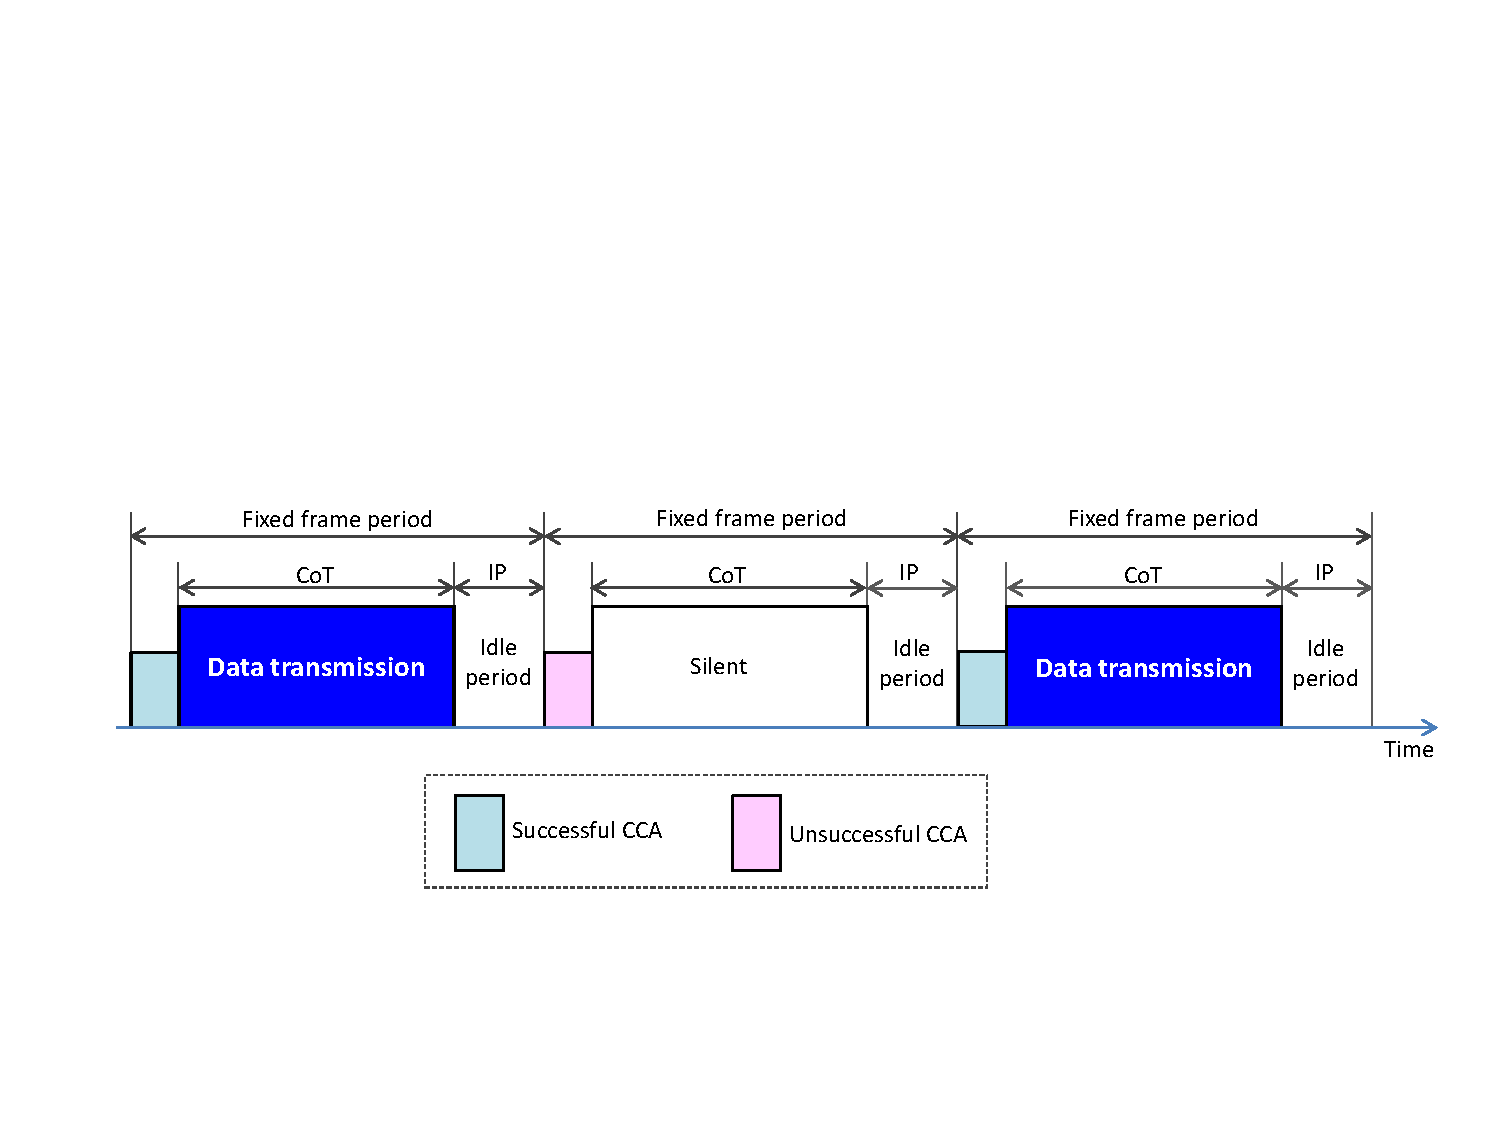
\includegraphics[width=0.9\columnwidth]{figures2/FBE-example}
\caption{An illustrative example of FBE.}
\label{figs:FBE-example}
\end{figure}

\subsubsection{FBE-based Mechanism}

FBE shall comply with the following requirements:

\begin{itemize}

\item
\textit{R1:} Before starting transmissions on an operating channel, the equipment shall perform a CCA check using Energy Detect (ED). The equipment shall observe the channel for the duration of the \textit{CCA observation time}. The operating channel shall be considered occupied if the energy level in the channel exceeds the \textit{threshold} corresponding to the power level.

\item
\textit{R2:}
If the CCA procedure finds the channel clear, the equipment may transmit immediately and occupy the channel for a \textit{fixed time period}.

\item
\textit{R3:} If the CCA procedure finds the channel occupied, the equipment shall not transmit on that channel during the next fixed frame period.

\item
\textit{R4:} The total time during which an equipment has transmissions on a given channel without re-evaluating the availability of that channel is defined as the \textit{Channel Occupancy Time} (CoT).

\item
\textit{R5:} After occupying the channel for CoT, the equipment keeps silent and waits for a short time, namely \textit{Idle Period} (IP).

\item
\textit{R6:} Towards the end of the idle period, the equipment shall perform a new CCA procedure as described in R1 above.

\item
\textit{R7:} The equipment, upon correct reception of a packet which was intended for this equipment, can skip CCA and immediately proceed with the transmission of management and control frames, e.g., acknowledgment (ACK) and block ACK frames.

\item
\textit{R8:}
A consecutive sequence of such transmissions by the equipment, without it performing a new CCA, shall not exceed the maximum CoT.

\item
\textit{R9:}
CCA observation time shall be not less than $20$ $\mu$s.

\item
\textit{R10:} CoT shall be in the range from $1$ ms to $10$ ms.

\item
\textit{R11:}
The minimum IP shall be at least $5$\% of CoT used by the equipment for the current fixed frame period.

\end{itemize}

A simplified flowchart and an illustrative of FBE are given in Figs. \ref{figs:FBE-flowchart} and \ref{figs:FBE-example}, respectively.



\begin{figure}[!t]
\centering
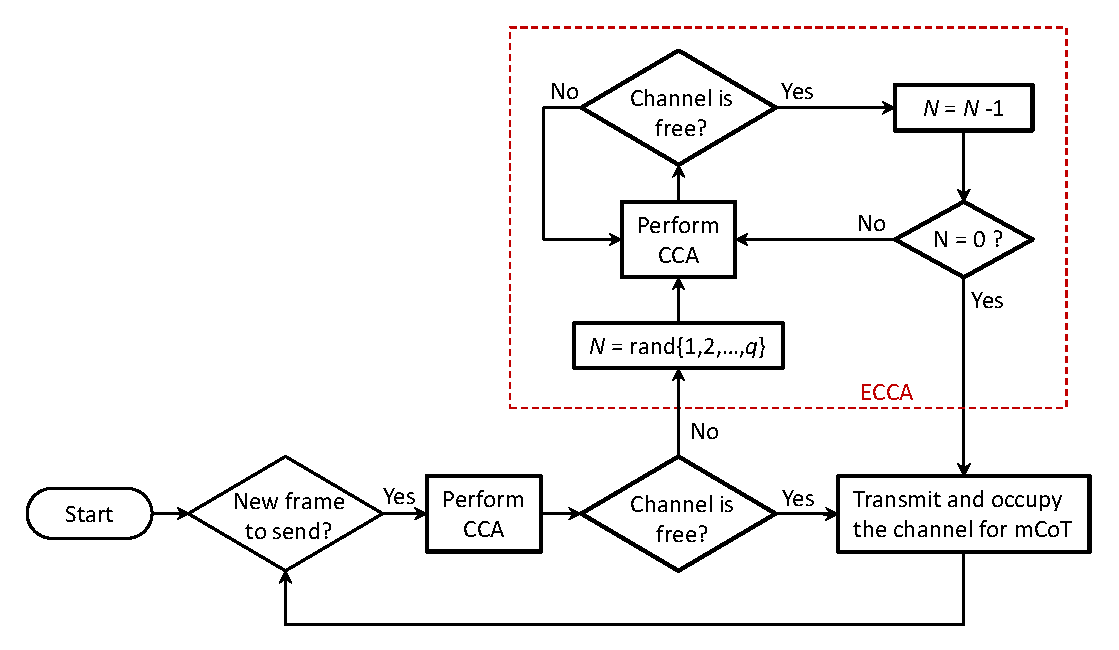
\includegraphics[width=0.9\columnwidth]{figures2/LBE-flowchart}
\caption{Simplified flowchart of LBE.}
\label{figs:LBE-flowchart}
\end{figure}

\begin{figure}[!t]
\centering
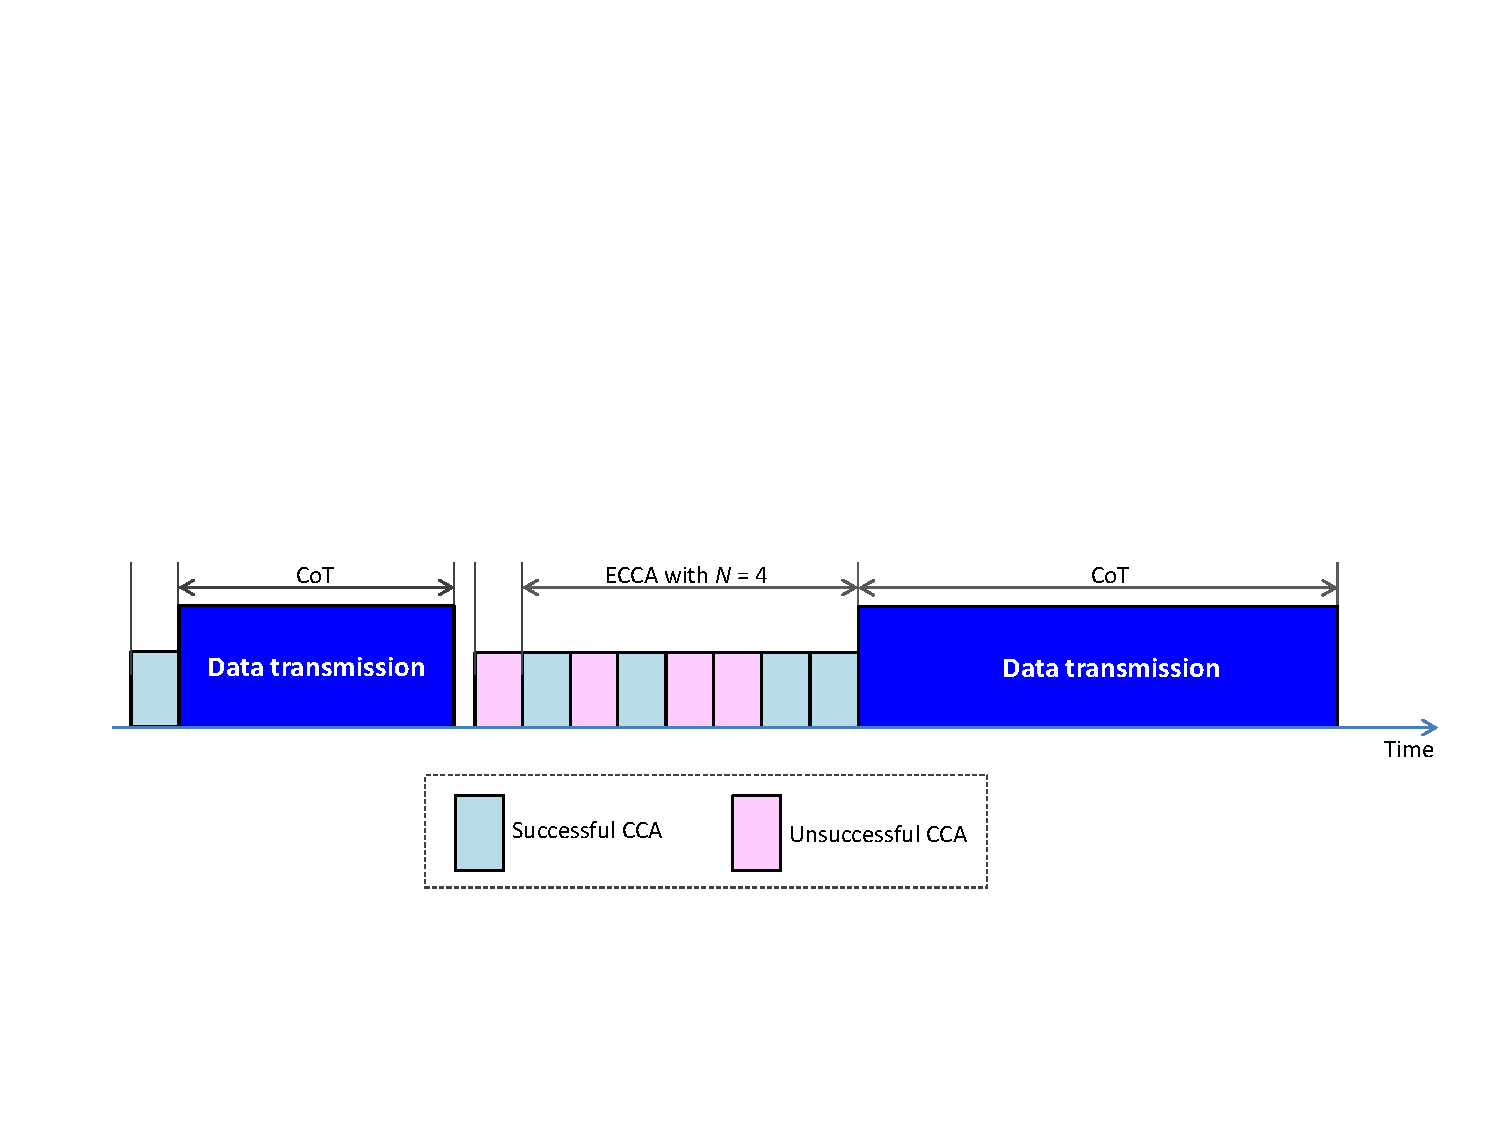
\includegraphics[width=0.9\columnwidth]{figures2/LBE-example}
\caption{An illustrative example of LBE.}
\label{figs:LBE-example}
\end{figure}

\subsubsection{LBE-based Mechanism}

LBE shall comply with the following requirements:

\begin{itemize}

\item
\textit{R1:} Before starting transmissions on an operating channel, the equipment shall perform a CCA check using ED. The equipment shall observe the channel for the duration of the \textit{CCA observation time}. The operating channel shall be considered occupied if the energy level in the channel exceeds the threshold corresponding to the power level.

\item
\textit{R2:}
If the CCA procedure finds the channel clear, the equipment may transmit immediately on that channel.

\item
\textit{R3:}
If the CCA procedure finds the channel occupied, it shall not transmit in that channel. The equipment shall perform an Extended CCA (ECCA) procedure in which the channel is observed for a random duration.

\item
\textit{R4:}
If the ECCA procedure has determined the channel to be clear, the equipment may start transmissions on this channel.

\item
\textit{R5:}
The total time that an equipment makes use of the channel (without performing CCA) is the \textit{maximum Channel Occupancy Time} (mCoT), after which the device shall perform a new CCA procedure as described in R1 above.

\item
\textit{R6:}
The equipment, upon correct reception of a packet which was intended for this equipment, can skip CCA and immediately proceed with the transmission of management and control frames, e.g., ACK and block ACK frames.

\item
\textit{R7:}
A consecutive sequence of transmissions by the equipment, without it performing a new CCA, shall not exceed mCoT.

\item
\textit{R8:}
CCA observation time shall be not less than $20$ $\mu$s.

\item
\textit{R9:}
The random duration in an ECCA procedure is $N \times$ (CCA observation time), where $N$ is randomly selected in the range $\{1,2,...,q\}$, $q \in \{4,5,...,32\}$ (declared by the manufacturer).

\item
\textit{R10:}
mCoT should be less than $(13/32)\times q$ ms (mCoT is in the range from $1.625$ to $13$ ms).

\end{itemize}

A simplified flowchart and an illustrative of LBE are given in Figs. \ref{figs:LBE-flowchart} and \ref{figs:LBE-example}, respectively.

\subsection{Wi-Fi's LBT Mechanism}

\begin{figure}[!t]
\centering
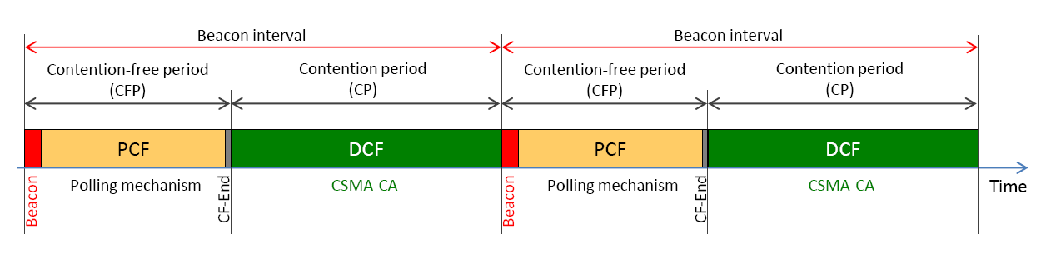
\includegraphics[width=1.0\columnwidth]{figures2/802-11-PCF-DCF}
\caption{PCF and DCF in IEEE 802.11.}
\label{figs:802-11-PCF-DCF}
\end{figure}


\section{An Overview of LTE Advanced}
\subsection{System Overview}
\subsubsection{Network Architecture}
\subsubsection{Capabilities and Features}
\subsection{Channel Access Mechanisms}
\subsubsection{LTE-A Physical Layer Protocol}
\subsubsection{LTE-A Medium Access Protocol}
\subsection{Changes Expected for Future Releases}
\subsubsection{An Overview on IEEE 802.11 and 802.11e}

\vspace{3mm}
\noindent $\bullet$ \textbf{IEEE 802.11 Basics}
\vspace{3mm}

\noindent The IEEE 802.11, a branch of 802 family of standards, defines the specifications of both physical and MAC layers of wireless local area networks (WLANs). The MAC layer is composed of two access modes: distributed coordination function (DCF) and point coordination function (PCF).

The first mode, DCF, is a contention-based LBT mechanism called \textit{Carrier Sense Multiple Access with Collision Avoidance (CSMA-CA)} that \textit{works in an entirely distributed manner without any coordination}. With CSMA-CA, stations (STAs) independently perform carrier sensing and back-off procedures to compete for the channel access. DCF is a mandatory MAC function and implemented in all IEEE 802.11/Wi-Fi devices. Details of CSMA-CA will be presented in subsection \ref{subsubsection:IEEE 802.11 CSMA-CA}.

The second mode, PCF, is built on the top of DCF. It aims to support applications that require near real-time services. Basically, PCF splits the time into periodic interval called beacon intervals, each of which is composed of contention-free period (CFP) and contention period (CP). \textit{CFP requires coordination from the access point (AP)} and allocates resources to STAs using polling mechanism. Specifically, AP maintains a list of registered PCF-enabled STAs and polls each of them using CF-Poll frames. Only after a STA is polled, it can start its data transmission. In case the polled STA does not have any frames to send, then it must transmit null frame. Channel access in CP of PCF is handled by CSMA-CA protocol. PCF is specified as an optional MAC function and has not been widely implemented due to its complexity.

The timing of PCF and DCF of IEEE 802.11 is sketched in Fig. \ref{figs:802-11-PCF-DCF}. Within a given beacon interval, the start and end of CFP are marked by beacon and CF-End control frames, respectively. CP follows CFP and is terminated by a beacon frame of the next beacon interval. The biggest limitation of IEEE 802.11 is its lack of capability to differentiate frames in terms of channel access priorities for different applications. As a result, the IEEE developed enhancements in IEEE 802.11e to both coordination modes to facilitate QoS.

\vspace{3mm}
\noindent $\bullet$ \textbf{IEEE 802.11e Basics}
\vspace{3mm}

\noindent The enhancement to DCF, namely Enhanced Distribution Coordination Function (EDCF), introduces the concept of
access categories (ACs). Each STA has four kinds of ACs that define four respective priority levels to differentiate the channel access probability for different traffic types. With EDCF, high priority traffic has a higher chance of being sent than low priority traffic: a STA with high priority traffic waits a little less before it sends its packet, on average, than a STA with low priority traffic. This is accomplished by using a shorter contention window and shorter Arbitration Interframe Space (AIFS).

IEEE 802.11e extends the polling mechanism of PCF with the Hybrid Coordination Function (HCF). The HCF controlled channel access (HCCA) works similarly to PCF. However, in contrast to PCF, in which the interval between two beacon frames is strictly divided into two periods of CFP and CP, the HCCA allows CFPs to be initiated at almost any time during a CP. This kind of CFP is called a Controlled Access Phase (CAP) in 802.11e. A CAP is initiated by the AP whenever it wants to send a frame to a STA or receive a frame from a STA in a contention-free manner. In fact, the CFP is a CAP too. During a CAP, the Hybrid Coordinator (HC), which is also the AP, controls the access to the medium using polling mechanism. During the CP, all STAs function in EDCA. The second difference with PCF is that Traffic Class (TC) and Traffic Streams (TSs) are defined. This means that HC is not limited to per-station queuing and can provide a kind of per-session service. Also, HC can coordinate these streams or sessions in any fashion it chooses (not just round robin). Moreover, STAs give information about the lengths of their queues for each TC. HC can use this information to give priority to one STA over another, or better adjust its scheduling mechanism.

IEEE 802.11e additionally introduces the concept of transmission opportunity (TXOP). A STA which obtains medium access must not utilize radio resource for duration longer than a limit specified by TXOP. The use of TXOPs reduces the problem of low-rate STAs gaining an inordinate amount of channel time in the conventional 802.11 DCF MAC. Another enhancement is that a STA is only allowed to initiate a frame exchange if it can complete the exchange before the start of the next beacon interval.

\begin{figure}[!t]
\centering
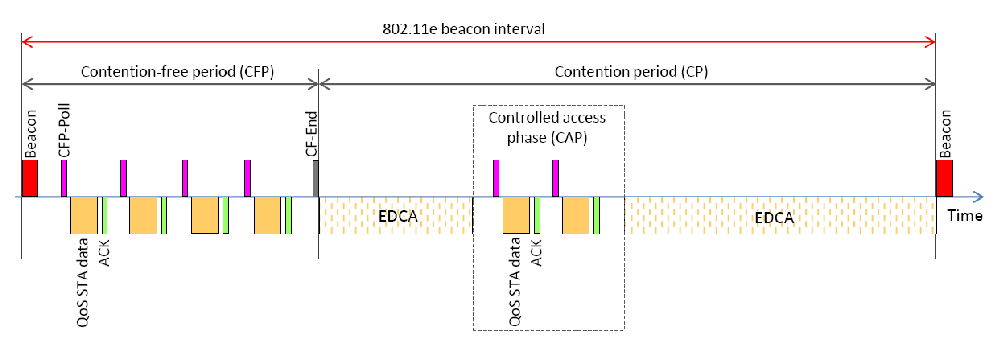
\includegraphics[width=1.0\columnwidth]{figures2/802-11e-HCCA}
\caption{HCCA in IEEE 802.11e.}
\label{figs:802-11e-HCCA}
\end{figure}

Basic operations of HCCA are illustrated in Fig. \ref{figs:802-11e-HCCA}. HCCA is generally considered as the most advanced and complicated coordination function. With HCCA, QoS can be configured with great precision. QoS-enabled STAs have the ability to request specific transmission parameters (data rate, jitter, etc.), which should allow advanced applications like voice over IP (VoIP) and video streaming to work more effectively on Wi-Fi networks. However, due to its complexity and signaling overhead, HCCA has not been widely implemented.

It can be seen IEEE 802.11 CSMA-CA is the most fundamental protocol for medium access in WLANs. In fact, IEEE 802.11e EDCA is primarily designed based on CSMA-CA. As a result, in-depth knowledge on medium access mechanisms employed by this protocol is imperative to understand and analyze the interactions between U-LTE and Wi-Fi networks when they operate in the same frequency band. To this end, technical details of CSMA-CA will be presented in the next subsection.

\subsubsection{IEEE 802.11 CSMA-CA}
\label{subsubsection:IEEE 802.11 CSMA-CA}

\vspace{3mm}
\noindent $\bullet$ \textbf{The Basic Channel Access}
\vspace{3mm}

\noindent The LBT mechanism employed by the IEEE 802.11/Wi-Fi CSMA-CA basically follows the same philosophy of carrier sensing protocol family: when a STA needs to transmit a new frame, the channel is sensed and if it is found idle the frame is transmitted immediately. This simple mechanism is very effective when the medium is not heavily loaded since it allows STAs to transmit with a minimum delay. However, it cannot prevent channel access collisions when multiple STAs detect free channel and decide to transmit their frames at the same time. As a result, in addition to this basic channel access, a number of important mechanisms are mandated in CSMA-CA.

\begin{figure}[!t]
\centering
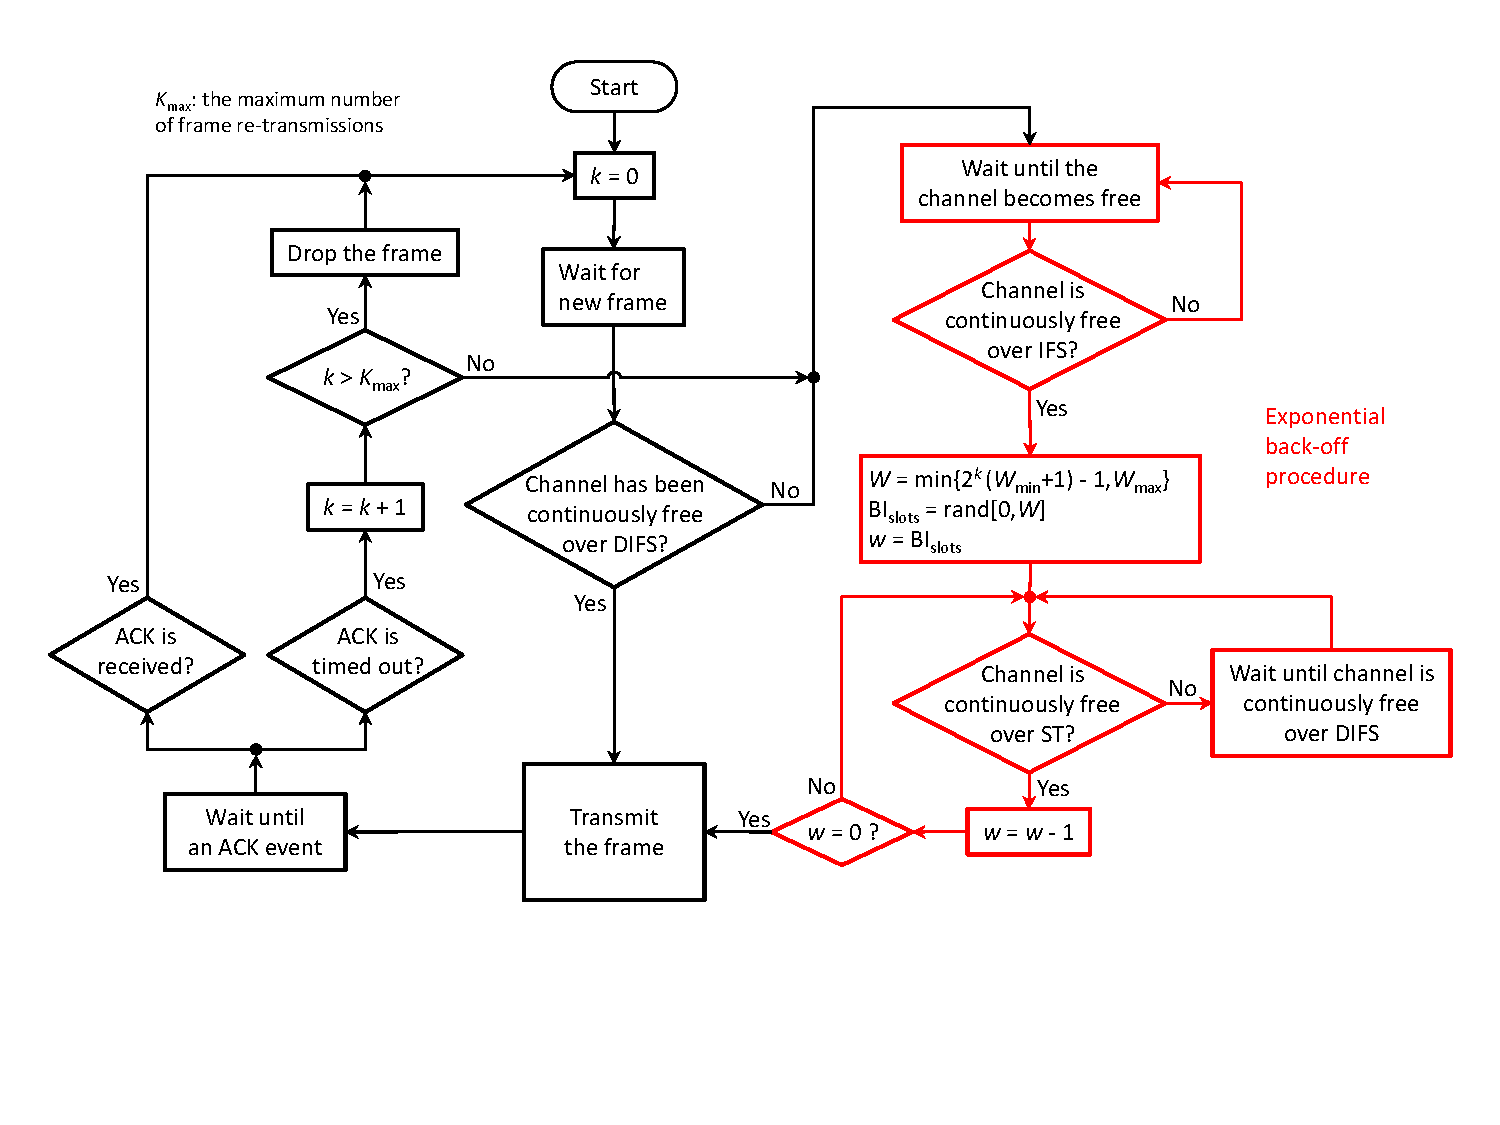
\includegraphics[width=1.0\columnwidth]{figures2/CSMA-CA-flowchart}
\caption{Simplified flowchart of CSMA-CA.}
\label{figs:CSMA-CA-flowchart}
\end{figure}

\vspace{3mm}
\noindent $\bullet$ \textbf{Channel Access with Collision Avoidance}
\vspace{3mm}

\noindent Since it is difficult to detect collisions at a wireless receiver, the IEEE 802.11 protocol tries to avoid collisions, rather than detect and recover from collisions. This means that CA mechanisms are mandated to reduce the collision probability at the points where collisions would most likely occur. Specifically, most collisions happen when the medium has become idle (as indicated by CS function) after a busy state: several STAs could have been waiting for the medium to be available again, then all transmit at the same moment the medium is detected free. This situation necessitates a ``random'' back-off procedure to resolve medium contention conflicts. Also, the use of various Inter-Frame Spaces (IFSs) helps to resolve the problem. The CSMA-CA protocol is outlined as follows.

\begin{figure}[!t]
\centering
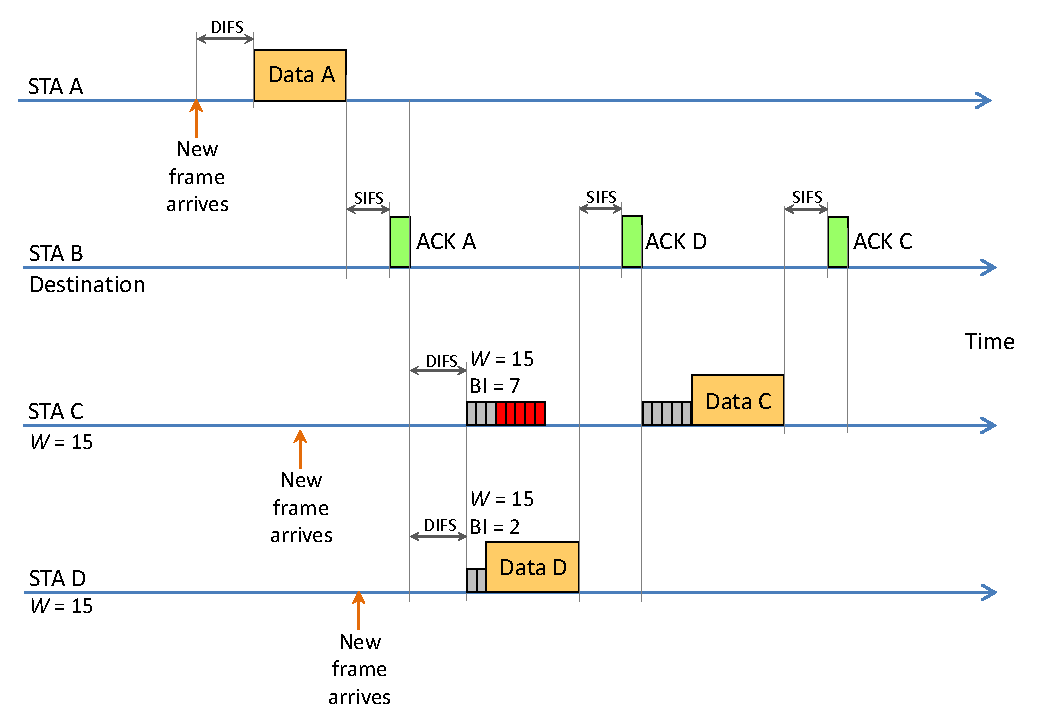
\includegraphics[width=0.9\columnwidth]{figures2/CSMA-CA-back-off-no-collision}
\caption{CSMA-CA: An example of back-off procedure when there is no collision.}
\label{figs:CSMA-CA-back-off-no-collision}
\end{figure}

When a STA needs to transmit a new frame, if the channel has been continuously free over a Distributed IFS (DIFS) interval, it transmits immediately. Otherwise, STA defers its transmission until the channel becomes available. Then if the channel is detected to be continuously free over a Distributed IFS (DIFS) interval, the STA will initiate the back-off procedure to further defer its transmission over a random time interval. The back-off procedure starts with the selection of a random ``slotted'' back-off interval $\mathrm{BI_{slots}} = \mathrm{rand}[0,W]$, where $\mathrm{rand}[0,W]$ is a random number uniformly distributed in the range from $0$ to $W$, $W$ is back-off window (when the system is started $W$ is assigned to its minimum value $W_{\min}$). Next, back-off counter $w$ is initialized with $\mathrm{BI_{slots}}$ and decreased every time the medium is idle over a Slot Time (ST). This counter is frozen when a transmission is detected on the medium, and resumed when the channel is detected idle again for a DIFS interval. As soon as $w$ finally reaches zero, the STA transmits its frame. It is important to note that this back-off procedure randomizes the channel access among STAs and thus helps to reduce the chance of collision. It also gives all STAs their fair shares of the channel.

The destination STA, upon receiving a frame correctly, waits for a Short IFS (SIFS) interval immediately after the reception has completed and transmits an ACK frame back to the source STA in order to confirm the correct reception. SIFS is the smallest IFS to give the highest priority channel access to ACK frames. If the source STA receives a confirmation, transmissions of the second and subsequent frames of a fragment burst will use SIFS instead of DIFS. Otherwise, the source STA activates the re-transmission procedure for the lost frame.

When a transmission is lost (due to channel collision when two or more STAs decrease their back-off counter to zero at the same time and transmit their frames at the same time or transmission errors), the contention window $W$ is doubled and applied for the re-transmissions until it reaches a maximum value $W_{\max}$. For the re-transmissions, the back-off procedure is activated after the channel remains idle for an Extended IFS (EIFS) interval. When a frame transmission is successful, contention window $W$ is reset to its minimum value $W_{\min}$. When a maximum number of frame re-transmissions is exhausted, the frame is discarded and $W$ is also reset to its minimum value $W_{\min}$.

\begin{figure}[!t]
\centering
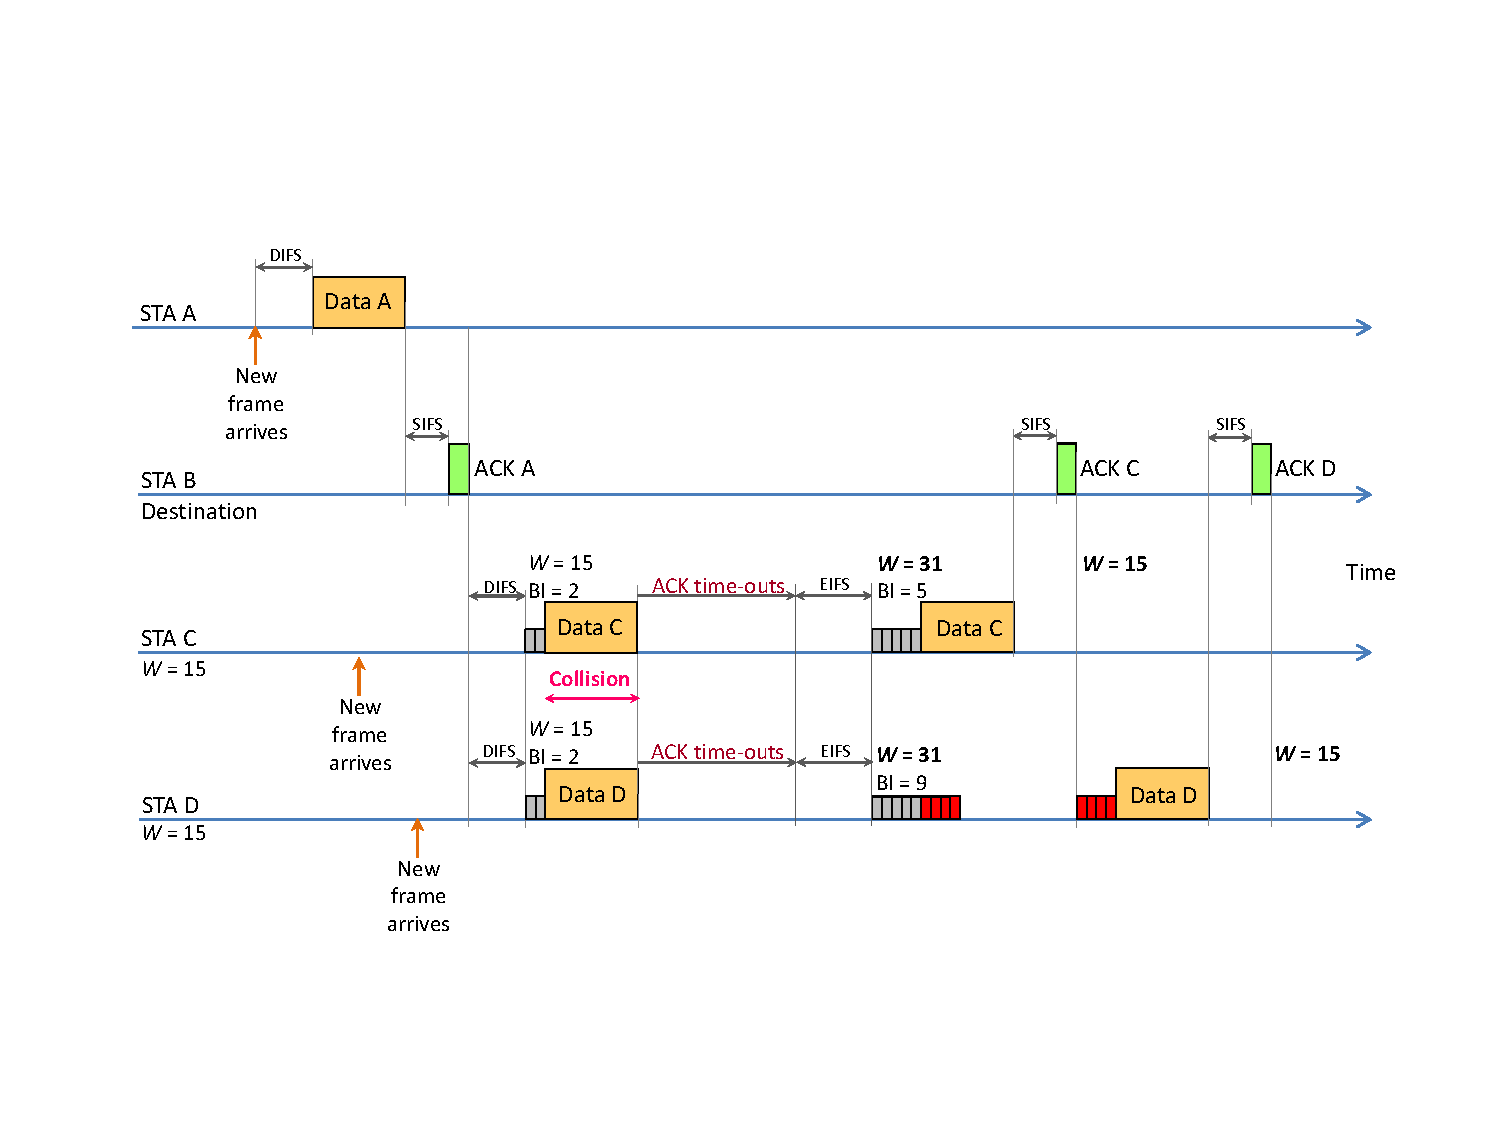
\includegraphics[width=1.0\columnwidth]{figures2/CSMA-CA-back-off-with-collision}
\caption{CSMA-CA: An example of back-off procedure when there is a collision (the contention window is exponentially increased).}
\label{figs:CSMA-CA-back-off-with-collision}
\end{figure}

The reason behind the exponential growth of contention window $W$ is explained as follows. When a STA experiences a collision, it has no information on how many STAs are involved in the collision. If there are only few colliding frames, it would make sense to choose the random back-off interval from a small set of small values, i.e., $W$ is small. But if many STAs are involved in a collision, then it makes sense to choose the back-off interval from a larger, more dispersed set of values, i.e., $W$ is large. Otherwise, if several STAs select the back-off interval from a small set of values, more than one STA would choose the same back-off value with high probability. This will result in high probability of collision.

Fig. \ref{figs:CSMA-CA-flowchart} shows the flowchart of CSMA-CA protocol. Figs. \ref{figs:CSMA-CA-back-off-no-collision} and \ref{figs:CSMA-CA-back-off-with-collision} demonstrates the operations of the back-off procedure in two typical scenarios. As visualized in Fig. \ref{figs:CSMA-CA-back-off-no-collision}, by randomly selecting back-off intervals, STAs C and D randomize their channel access to minimize the chance that they transmit their frames at the same time. In case a collision takes place, as shown in Fig. \ref{figs:CSMA-CA-back-off-with-collision}, STAs C and D double their contention windows to further increase the randomness in their back-off interval generations.

Here are some illustrative values of CSMA-CA operation parameters: ST = $20$ $\mu$s, SIFS = $10$ $\mu$s, DIFS = SIFS + $2\times$ST = $50$ $\mu$s, EIFS = Transmission time of ACK frame at lowest physical mandatory rate + SIFS + DIFS, $W_{\min}$ = $31$, and $W_{\max}$ = $1023$. Contention window of the initial transmission attempt is $W(0)=W_{\min}=31$. Contention window of the $k$-th re-transmission is $W(k)=\min\{2^{k}(W_{\min}+1)-1, W_{\max}\}$, where $k \in \{1,2, ..., K_{\max}\}$, $K_{\max}$ is the maximum number of re-transmission attempts. Assuming $K_{\max}=7$, then the progression of contention window with frame transmission/re-transmissions is as follows: $W(0)=31$ (the initial transmission attempt), $W(1)=63$ (the first re-transmission attempt), $W(2)=127$ (the second re-transmission attempt), $W(3)=255$ (the third re-transmission attempt), $W(4)=511$, $W(5)=1023$, $W(6)=1023$, and finally $W(7)=1023$. Different IEEE 802.11 physical layer standards could specify different values for these parameters to optimize their operations.

\begin{figure}[!t]
\centering
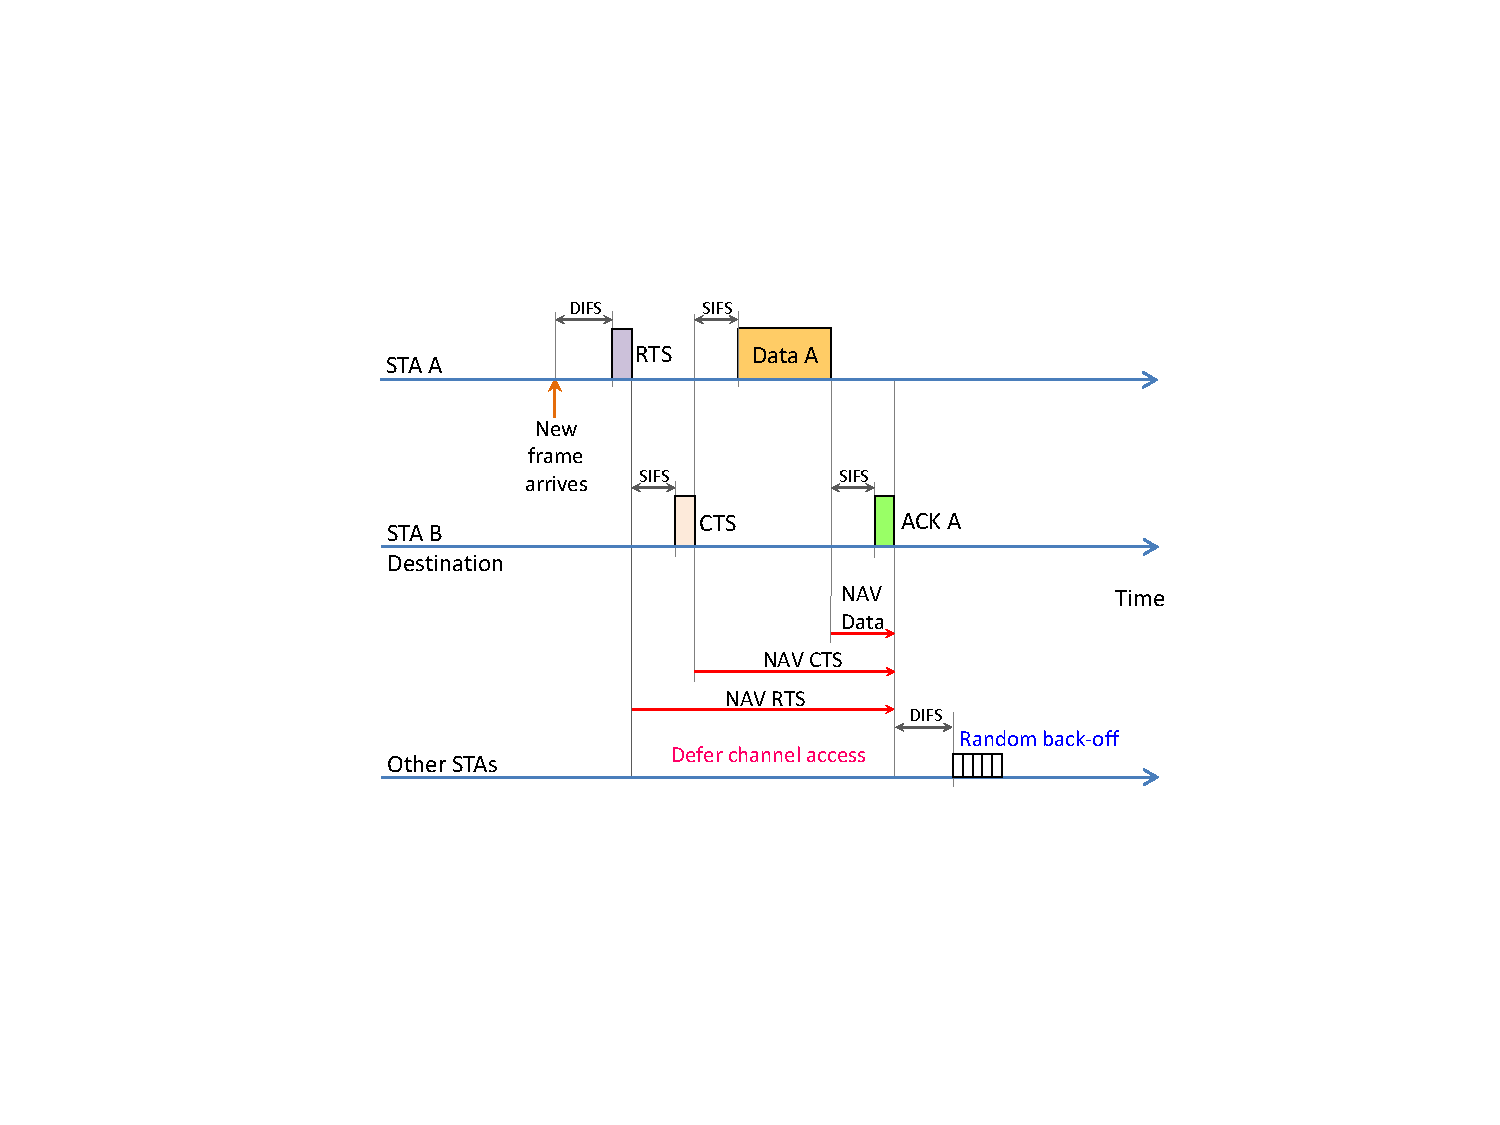
\includegraphics[width=0.65\columnwidth]{figures2/802-11-RTS-CTS-NAV}
\caption{CSMA-CA enhanced with RTS/CTS handshake and NAV.}
\label{figs:802-11-RTS-CTS-NAV}
\end{figure}

\vspace{3mm}
\noindent $\bullet$ \textbf{Enhanced Collision Avoidance}
\vspace{3mm}

\noindent In order to provide guaranteed reservation of the channel and hence uninterrupted data transmission, CSMA-CA protocol can be enhanced with Request-To-Send (RTS)/Clear-To-Send (CTS) handshake and virtual carrier sense using Network Allocation Vector (NAV). The former is an optional mechanism and only employed for transmissions of long frames (determined by RTS threshold which is typically around $500$ bytes). The latter is a prominent mechanism which is widely used with CSMA-CA protocol.

In RTS/CTS access mode, prior to the data transmission, the source STA will send a RTS frame to announce the upcoming transmission. When the destination STA receives RTS, it will send a CTS frame after a SIFS interval if it is available to receive the data. The source STA is allowed to transmit its data frame only if it receives the CTS frame correctly. The purpose of this RTS/CTS exchange is to clear hidden areas and avoid long collisions. RTS/CTS is illustrated in Fig. \ref{figs:802-11-RTS-CTS-NAV}.

To implement virtual carrier sensing, each STA sends duration information in frame headers. This duration information indicates the amount of time (in microseconds) the medium is to be reserved after the end of the current frame. STAs listening on the wireless medium read the duration fields and set their NAVs, which is an indicator for a STA on how long it must defer from accessing the medium. They count down their NAVs and do not access the channel (even if their physical carrier sense indicates that the channel is free) until NAVs reach zero. NAV is illustrated in Fig. \ref{figs:802-11-RTS-CTS-NAV}. As can be seen, the NAV field in RTS frame allows CTS, data, and ACK frames to be completed (or allows only CTS frame to be completed in some implementations). The NAV in CTS frame allows data and ACK frames to be completed. Finally, the NAV in data frame allows the ACK frame to be completed.

\subsubsection{Important Observations on IEEE 802.11 CSMA-CA}

It is important to note that IEEE 802.11 CSMA-CA is specified with a few key additional features that go beyond LBT requirements specified by ETSI \cite{LBT-ETSI-2014}. \textit{First}, a Wi-Fi device defers to signals that are much weaker than the minimum level required by ETSI. ETSI LBT requires a transmitter to defer if the received energy is above $-60$ dBm (for $20$ MHz), while Wi-Fi defers if the received energy is above $-62$ dBm (this level is referred to as the energy detect threshold, or ED for short) or if a valid Wi-Fi preamble is detected. Wi-Fi's ED threshold is nearly the same as ETSI's LBT threshold, but Wi-Fi preamble detection is required to work to at least $-82$ dBm, and in reality works to $-90$ dBm or lower in most products. Hence, Wi-Fi devices defer to other Wi-Fi transmissions much more conservatively (i.e., at a much larger distance) than a device which only meets ETSI requirements. \textit{Second}, Wi-Fi goes beyond the ETSI requirements in specifying how long a device must wait after the on-air energy falls below the threshold before initiating a transmission. \textit{Third}, when a collision is detected, Wi-Fi employs exponential back-off rule that doubles the contention window size and thus significantly increases the random back-off time in order to avoid future collision.


%**************************************************************************************************************%
\section{An Overview on LTE-U and LAA-LTE}
\label{sec:U-LTE-overview}

\subsection{LTE-U}

\noindent This is the simplest form of U-LTE that requires minor modifications in LTE protocol stack. Therefore, it can quickly facilitate pre-standard equipment manufacturing and deployment. LTE-U first attempts to select clear channel to access. If no clear channel is found, it will employs Carrier-Sensing Adaptive Transmission (CSAT) which is a Time-Division Multiplex (TDM) coexistence based on medium sensing. CSAT employs ``duty-cycling'' instead of LBT mechanism. Compared to LBT or CSMA, the small cell senses the medium for a longer duration (around $10$s of millisecond to $200$ millisecond) and according to the observed medium activities, the algorithm gates off LTE transmission proportionally. In particular, CSAT defines a time cycle where the small cell transmits in a fraction of the cycle and gates off in the remaining duration. The duty cycle of transmission versus gating off is dictated by the sensed medium activity of neighboring RANs. The TDM cycle can be set to a few tens or hundreds of millisecond, which can effectively accommodate the activation/de-activation procedures while controlling the data transmission delay. CSAT is illustrated in Fig. \ref{figs:LTE-U}. An important observation from Fig. \ref{figs:LTE-U} is that during the LTE ``on'' period, Wi-Fi is blocked by LTE-U transmissions. During the LTE ``off'' period, Wi-Fi will detect that the channel is free and can schedule its transmissions following its CSMA-CA protocol.

LTE-U is only applicable in areas where there are no strict LBT requirements for operations in unlicensed bands (e.g., US. Korea, China). It is a non-standard version of U-LTE, being developed outside of the 3GPP standards process. LTE-U is supported by LTE-U Forum formed in 2014 by Verizon in cooperation with Alcatel-Lucent, Ericsson, Qualcomm Technologies Inc. (a subsidiary of Qualcomm Incorporated), and Samsung.

\begin{figure}[!t]
\centering
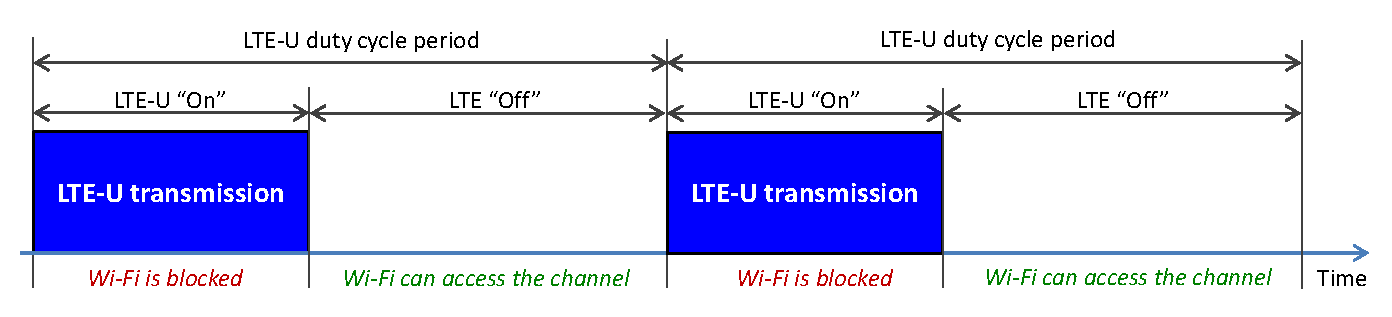
\includegraphics[width=0.95\columnwidth]{figures2/LTE-U}
\caption{Duty-cycling mechanism employed by LTE-U.}
\label{figs:LTE-U}
\end{figure}

\subsection{LAA-LTE}
\label{subsection:LAA-LTE}

\noindent In many areas such as Europe, Japan and India, there exist regulations for unlicensed spectrum that require equipment to periodically check for presence of other occupants in the channel, so-called LBT, in millisecond scale. LAA-LTE is designed for use in those areas or for global use. It requires a number of modifications so that LTE transmissions can meet regulatory requirements in LBT regions. Similar to LTE-U, LAA-LTE first tries to choose the cleanest channel based on Wi-Fi and LTE measurements to operate on. In the event that no clean channel is available, LBT algorithm is used to compete the medium with other RANs in the same channel. For LBT, FBE- and LBE-based mechanisms specified in \cite{LBT-ETSI-2014} have been used. Details of these two mechanisms have been presented in section \ref{subsec:ETSI-LBT-overview}.

Assuming that LBE-based LBT is employed for LAA-LTE. Before transmission, CCA using ED is performed. If the channel is clear during a CCA slot ($20$ microseconds or longer), transmission is started immediately. Otherwise, ECCA is performed. If the channel is clear during $N$ CCA slots, transmission is started immediately. $N$ is a random integer uniformly distributed from $1$ to $q$, where $q \in \{4,5,...,32\}$. The total time to occupy the channel without CCA is limited by $(13/32)q$ milliseconds (e.g., $13$ milliseconds when $q$ is $32$). Two simplified scenarios with LAA-LTE (employing LBE-based LBT) and Wi-Fi systems operating in the same channel are illustrated in Fig. \ref{figs:LAA-LTE}. In the first scenario, the LAA-LTE system, upon having data frames to send, performs CCA and then ECCA (with $N=7$) since there is an ongoing Wi-Fi transmission. The ECCA procedure is frozen and then resumed when another Wi-Fi transmission takes place and then completes, respectively. The LAA-LTE system finally transmits its frames once ECCA counter $N$ reaches zero. In the second scenario, the Wi-Fi system, upon having data frames to send, performs CCA and then back-off procedure (with $\mathrm{BI_{slots}} = 7$) since there is an ongoing LAA-LTE transmission. The back-off procedure is frozen and resumed when another LAA-LTE transmission takes place. The Wi-Fi system finally transmits its frames once back-off counter $w$ reaches zero.

LTE was originally designed for licensed spectrum and a centralized management (i.e., network-controlled) model, it is generally an ``always-on'' technology. As a result, adapting to LBT is a marked change for the LTE protocol. Compared to LTE-U which is downlink-only in unlicensed bands, LAA-LTE may allow bi-directional traffic in unlicensed bands.

LAA-LTE is currently actively supported by 3GPP and will be included in 3GPP LTE Release 13 (to be published by March 2016). T-Mobile USA and Verizon Wireless have indicated their interests in deploying pre-standard LAA-LTE systems for evaluations and commercial services in 2016.

\begin{figure}[!t]
\centering
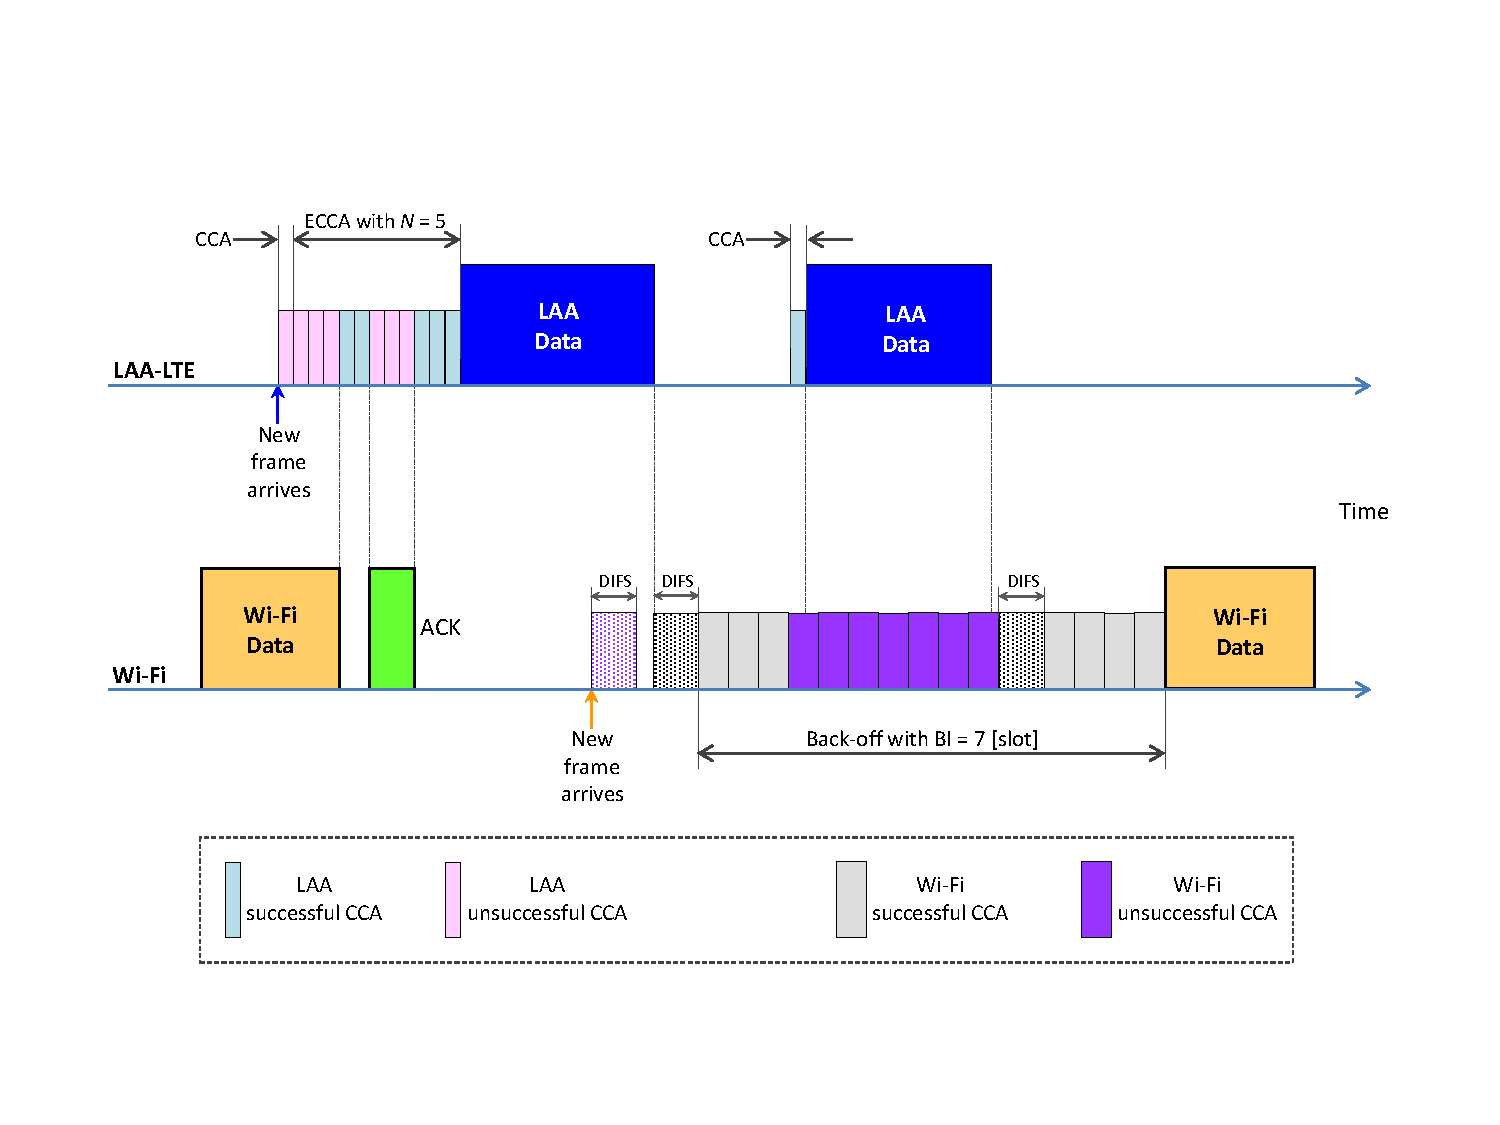
\includegraphics[width=0.9\columnwidth]{figures2/LAA-LTE}
\caption{CCA and ECCA mechanisms employed by LAA-LTE.}
\label{figs:LAA-LTE}
\end{figure}


%**************************************************************************************************************%

\section{A Survey on Related Work}
\label{sec:relatedwork}

\noindent So far, there have not been many papers in this research area. Most of them attempt to identify what could be the affects that U-LTE may cause to Wi-Fi networks and which mechanisms could be used for coexistence between them. More specifically, they address the following questions: (i) what issues arise from simultaneous operation of LTE and Wi-Fi in the same spectrum bands, (ii) what technology is affected the most, (iii) how different factors determine the effects of U-LTE to Wi-Fi, and (iv) what could be appropriate strategies to improve performance of both networks while coexisting. A number of surveys on U-LTE can be found in \cite{U-LTE-survey-2014, U-LTE-survey-2015, U-LTE-5G-2015}.

Most existing works dealing with U-LTE carry out studies by using system-level simulations. A few of them use analysis or experiments (using off-the-shelf devices and radio development platforms). Two types of U-LTE approaches are considered: LTE-U and LAA-LTE. Coexistence mechanisms considered include: Dynamic Channel Selection (DCS), power control, opportunistic secondary cell ``off'', CSAT (in LTE-U), and LBT (in LAA-LTE). The followings present a survey on related works that can be generally categorized into four main groups focusing on: (i) investigations on how original (unmodified) LTE can affect Wi-Fi, (ii) concerns on U-LTE and requests for further studies, (iii) mechanisms and reasons to support U-LTE, and (iv) combinations of these focuses.

In \cite{original-LTE-Wi-Fi-VTC-2013}, extensive simulations have been performed to assess the performance of LTE and Wi-Fi coexisting in an office environment. Single-floor and multi-floor office environments with different assumptions on the density of Wi-Fi and LTE nodes have been considered. The simulation results in \cite{original-LTE-Wi-Fi-VTC-2013} have shown that, in the absence of any modification to LTE channel access mechanism, channel sharing between LTE and Wi-Fi networks is significantly unfair for Wi-Fi networks. While LTE only marginally loses (about $4$\% of the performance) when Wi-Fi is present on the same band, Wi-Fi could lose up to $70$\% performance in a sparse deployment ($1$ AP per system per floor) and to almost $100$\% in a dense deployment ($5$ APs per system per floor). Detailed investigations in \cite{original-LTE-Wi-Fi-VTC-2013} have indicated that Wi-Fi channel is blocked when LTE interference is present, and thus Wi-Fi nodes keep staying on the ``listen'' mode most of the time.

The authors in \cite{original-LTE-Wi-Fi-WCNC-2013} present observations similar to those in \cite{original-LTE-Wi-Fi-VTC-2013} on the effects of unmodified LTE to Wi-Fi networks in the shared frequency band. Specifically, when network load is increased, LTE performance suffers only a minor degradation, while Wi-Fi performance drops significantly. This can be explained by the increasing LTE occupancy on the shared band. LTE does not follow the same rules as Wi-Fi in shared medium access. When there is ongoing transmission on the channel, while Wi-Fi politely defers its transmission, LTE always choose to transmit by selecting a more robust transmission mode by adapting its modulation and channel coding scheme in order to cope with the higher interference. This aggressive behavior quickly results in a situation where LTE terminals take all transmission opportunities while Wi-Fi devices are locked in back-off procedures. Unfortunately, the results in \cite{original-LTE-Wi-Fi-WCNC-2013} have also demonstrated that the severity of this negative impact on Wi-Fi can be efficiently controlled by restricting LTE activity.

The authors in \cite{LTE-U-PIMRC-2014} analyze the performance degradation of Wi-Fi in the presence of LTE-U. The probability of Wi-Fi accessing the channel is used as the main metric. Numerical results in \cite{LTE-U-PIMRC-2014} indicate that Wi-Fi is negatively affected by conventional LTE operation due to LTE's almost continuous transmission that subsequently blocks Wi-Fi. Specifically, given two modes of operations currently proposed for LTE-U in the unlicensed spectrum, the ``off'' period presented by the LTE protocol is too short for Wi-Fi users to access to the channel. As a result, Wi-Fi is at risk of spending a significant amount of time in the ``listening'' mode when LTE transmission is present in the same channel.

The work in \cite{U-LTE-Google-WP} presents initial investigations on the coexistence of two versions of license-anchored U-LTE (i.e., LTE-U and LAA-LTE) and Wi-Fi in $5$ GHz frequency band. Results in \cite{U-LTE-Google-WP} show that LTE-U poorly coexists with Wi-Fi primarily due to two factors: (i) the incompatibility of LTE-U's duty-cycling mechanism with Wi-Fi equipment and (ii) the lack of an effective coexistence mechanism in scenarios where LTE-U and Wi-Fi devices hear each other at moderate but non-negligible power levels. Additionally, LAA-LTE with LBT does not by itself guarantee successful coexistence with Wi-Fi and other purely unlicensed technologies. The results in \cite{U-LTE-Google-WP} were submitted to FCC in June 2015 to demonstrate that, although any wireless technology should have the ability to utilize unlicensed spectrum within the FCC's rules, U-LTE has the potential to crowd out unlicensed services.

An experiment-based study on the effect of LTE-U to Wi-Fi is presented in \cite{LTE-U-CableLabs}. The LTE signal level is set higher than the Wi-Fi clients' LBT energy detection threshold (i.e., when LTE is on, the Wi-Fi client should sense their presence and not transmit). Wi-Fi throughput and latency are measured when data is transmitted through the Wi-Fi network with varying duty cycles and periods of LTE signals. The results in \cite{LTE-U-CableLabs} indicate that, as expected, increasing the LTE-U duty cycle degrades both Wi-Fi throughput and latency performance since it decreases Wi-Fi transmission opportunity accordingly. If the duty cycle period is too high, Wi-Fi latency is negatively impacted (while Wi-Fi throughput is nearly unchanged, given the same duty cycle) since Wi-Fi frames have to be buffered during long LTE ``on'' period. However, if the duty cycle period is configured as too low (e.g., $10$ msec), Wi-Fi throughput degrades due to the fact that LTE ``on'' and ``off'' periods are too short for Wi-Fi users to access to the channel and to complete their transmissions, respectively. Furthermore, the authors in \cite{LTE-U-CableLabs} indicate that LTE-U duty cycle cannot strictly results in corresponding air time and throughput sharings. For example, with a duty cycle of $50$\%, LTE-U is likely to capture more than $50$\% of the channel resources. The reason is that when LTE-U starts its transmissions (regardless of ongoing Wi-Fi frame transmissions), many Wi-Fi frames are corrupted. Transmission failures lead to multiple frame re-transmissions and, more importantly, mistakenly force Wi-Fi transceivers to operate at lower rates (in this case, lowering the channel coding and modulation modes is not necessary and waste of channel efficiency).

In order to see how LBT mechanisms employed by LAA-LTE can help for the coexistence, a simulation-based study is carried out and reported in \cite{LBT-CableLabs-2014}. LBE LBT specified by ETSI \cite{LBT-ETSI-2014} and IEEE 802.11e Enhanced Distributed Channel Access (EDCA) are assumed for LAA-LTE and Wi-Fi, respectively. The most important observation from \cite{LBT-CableLabs-2014} is that LBT compliant to ETSI regulation is not sufficient for fair coexistence: Wi-Fi STAs have much lower probability of successful channel access compared to LAA-LTE users. One major reason for this phenomenon is the non-exponential back-off LBT employed by LAA-LTE. Unfortunately, no form of exponential back-off LBT is studied in \cite{LBT-CableLabs-2014}.

In \cite{U-LTE-Wi-Fi-Qualcomm-2014, LTE-U-Wi-Fi-LTE-U-Forum-2015, LTE-U-Qualcomm-2015, U-LTE-Wi-Fi-Qualcomm-FCC-2015}, the performance of LTE-U and LAA-LTE and Wi-Fi in a shared frequency band is evaluated. DCS and opportunistic secondary cell ``off'' in unlicensed spectrum (U-LTE small cells would release the unlicensed carriers and fall back to the anchor carrier in licensed spectrum at low traffic load) are jointly used with CSAT and LBT. The results show that co-existence has a negative but controllable impact on Wi-Fi performance. In \cite{U-LTE-Wi-Fi-Qualcomm-2014, LTE-U-Wi-Fi-LTE-U-Forum-2015, LTE-U-Qualcomm-2015}, LTE-U can be a better neighbor to Wi-Fi than Wi-Fi to itself in some scenarios. The underlying design that allows LTE-U to achieve high spectral efficiency while being a good neighbor to Wi-Fi is achieved through a set of carefully designed coexistence techniques, including DCS, secondary cell ``duty cycle'' in unlicensed spectrum (i.e., CSAT), and opportunistic secondary cell ``off'' in unlicensed spectrum. Specifically, in scenarios where the density of Wi-Fi APs and small cells is low or moderate, DCS and opportunistic secondary cell ``off'' are sufficient to meet the coexistence requirement. When LTE-U devices replace Wi-Fi devices, they can achieve significantly higher throughputs due to their high spectral efficiency. In addition, the performance of neighboring Wi-Fi is unchanged or even slightly improved since LTE-U devices can finish transmission faster and incur less interference. However, as the density of Wi-Fi devices and LTE-U small cells is high, DCS and opportunistic secondary cell ``off'' alone cannot guarantee harmonious coexistence with Wi-Fi and therefore CSAT or LBT is required. Resutls in \cite{LTE-U-Wi-Fi-LTE-U-Forum-2015, U-LTE-Wi-Fi-Qualcomm-FCC-2015} were submitted to FCC in 2015 to support U-LTE technologies.

A systematic and large-scale network-wide study of LAA-LTE and Wi-Fi performance in a wide range of realistic deployment scenarios and network densities in the unlicensed $5$ GHz band is presented in \cite{LTE-U-ICC-WS-2015}. The simulation results in all considered coexistence scenarios demonstrate that both LAA-LTE and Wi-Fi significantly benefit from the large number of available channels and the isolation provided by building shielding at $5$ GHz. They also suggest that deploying LAA-LTE with a random channel selection scheme is feasible for lower network densities. For typical indoor deployments of high density, implementing LTE-U interference-aware channel selection with respect to Wi-Fi is superior to LBT in terms of achieved throughput for both technologies. Additionally, LBT can increase LAA-LTE user throughput when multiple outdoor LAA-LTE networks deployed by different cellular operators coexist.

The work in \cite{Enhanced-LTE-U-thesis-2015} investigates the behavior and performance of two existing LBT mechanisms that are designed following the coexistence standard specified by ETSI \cite{LBT-ETSI-2014}: LBE and FBE-based mechanisms. The Jain's fairness index has been used to access the coexistence of LAA-LTE using these two LBT mechanisms and Wi-Fi using CSMA-CA. The simulations in \cite{Enhanced-LTE-U-thesis-2015} show that FBE-based mechanism using fixed contention window penalizes the channel access opportunity of Wi-Fi's CSMA-CA using adaptive contention window. They also reveal that FBE-based mechanism tends to aggressively occupy the channel. In some cases, Wi-Fi is starved with very less (or even no) chance on the channel access. This poor fairness is mainly caused by the short CCA sensing period of FBE-based mechanism. CCA is applied only once and then FBE-based mechanism may start its transmission immediately while LBE and Wi-Fi-based mechanisms are still decrementing their respective back-off counters. The fairness is worsened with longer FBE's frames. Another observation is that, again due to equal CCA sensing time, when multiple FBE-based equipment are contending for the channel, they are prone to serious collisions (if they are accidentally synchronized) or suffer a significant unfairness (if they are asynchronous). To cope with those issues, tuning the values of back-off scaler ($q$) to extend the contention window size and using CCA procedure similar to that of LBE-based mechanism have been suggested for LBE and FBT-based mechanism, respectively. The results in \cite{Enhanced-LTE-U-thesis-2015} demonstrate that the modified LBE-based mechanism still cannot sufficiently improve the fairness with others. This could be because simply empirically tuning back-off scaler while keeping the CCA principle unchanged cannot compensate for exponential growth of window size adopted by Wi-Fi's CSMA-CA. The modified FBE-based mechanism can offer better fairness when coexisting with Wi-Fi.

A comparison of LTE-U and LAA-LTE is presented in \cite{LBT-CSAT-2015}. The analysis in \cite{LBT-CSAT-2015} shows that for sufficiently long LTE transmission times, the LTE throughputs achieved by CSAT and LBE are almost identical. However, for shorter LTE transmission times, LTE-U provides lower LTE throughput than LAA-LTE due to higher LTE/Wi-Fi collision probability of LTE-U. Besides, while shorter LTE transmission time decreases the tail of the Wi-Fi delay distribution, the percentage of packets that suffer from long delays increases. The results also indicate that when appropriately configured, LTE-U and LAA-LTE provide the same level of fairness to Wi-Fi. The selection of co-existence mechanisms is primarily driven by the operator's interests that include implementation complexity, LTE throughput, operational and management costs as well as strategic decisions on targeted markets.

Coordinated coexistence between U-LTE and Wi-Fi is investigated in \cite{U-LTE-5G-2015, Coordinated-LTE-U-Wi-Fi-2015}. The authors in \cite{U-LTE-5G-2015} propose a method of centralized system management to combine LTE-U and Wi-Fi through network function virtualization (NFV) interconnections. It may enable seamless transfer of resources between LTE-U and Wi-Fi using in-the-cloud control of distributed access points. \textit{However}, only \textit{conceptual} network architectures and mechanisms are presented \cite{U-LTE-5G-2015}. The authors in \cite{Coordinated-LTE-U-Wi-Fi-2015} present a Software Defined Networking (SDN) architecture to support logically-centralized dynamic spectrum management involving multiple autonomous networks to improve spectrum utilization and facilitate co-existence. The basic design goal is to support the seamless communication and information dissemination required for coordination of heterogeneous networks. The system consists of two-tiered controllers are mainly responsible for the control plane. Global Controller (GC) acquires and processes global network state information (radio coverage maps, coordination algorithms, policy and network evaluation matrices, etc.) and controls the flow of information between RCs and databases based on authentication and other regulatory policies. Regional Controllers (RCs) acquire local visibility needed for radio resource allocation at wireless devices: device location, frequency band, duty cycle, power level, and data rate, etc. Joint power control and time division channel access optimizations are proposed. Analytical results in \cite{Coordinated-LTE-U-Wi-Fi-2015} demonstrate that, \textit{with full buffer traffic assumption}, centralized optimization approaches can provide fair access to the spectrumfor LTE-U and Wi-Fi networks.

An experimental evaluation of U-LTE interference effects on Wi-Fi performance under various network conditions along with some suggestions for better coexistence of U-LTE and Wi-Fi networks are presented in \cite{LTE-U-Experiment-ICC-WS-2015}. Various system parameters (bandwidth, center frequency, etc.) are swept to identify the most significant ones that determine the levels of LTE interference introduced to Wi-Fi carrier sense and performance. The results indicate that Wi-Fi throughput can be heavily degraded by LAA-LTE transmissions with $3$/$5$/$10$ MHz bandwidth (especially $3$/$5$ MHz). Besides, LAA-LTE transmissions can have small impact on Wi-Fi throughput when using a $1.4$ MHz channel with center frequencies located on the guard bands or the center frequencies of Wi-Fi channels. However, the authors in \cite{LTE-U-Experiment-ICC-WS-2015} do not clearly define what LAA-LTE really mean in their work. It seems to be that they simply perform experiments with conventional LTE transceivers of varying power spectral densities and do not incorporate any coexistence mechanism into the LTE system.

\section{Network-aware Adaptive Listen Before Talk Co-existence Mechanism}
\subsection{Background and Theoretical Basis}
\subsection{The Proposed Mechanism}
\subsection{Performance Evaluation}
\subsubsection{System Model}
\subsubsection{Simulation Results}
\subsection{Discussion and Future Work}


%**************************************************************************************************************%

\section{Open Questions and Potential Research Directions}
\label{sec:directions}

\begin{figure}[!t]
\centering
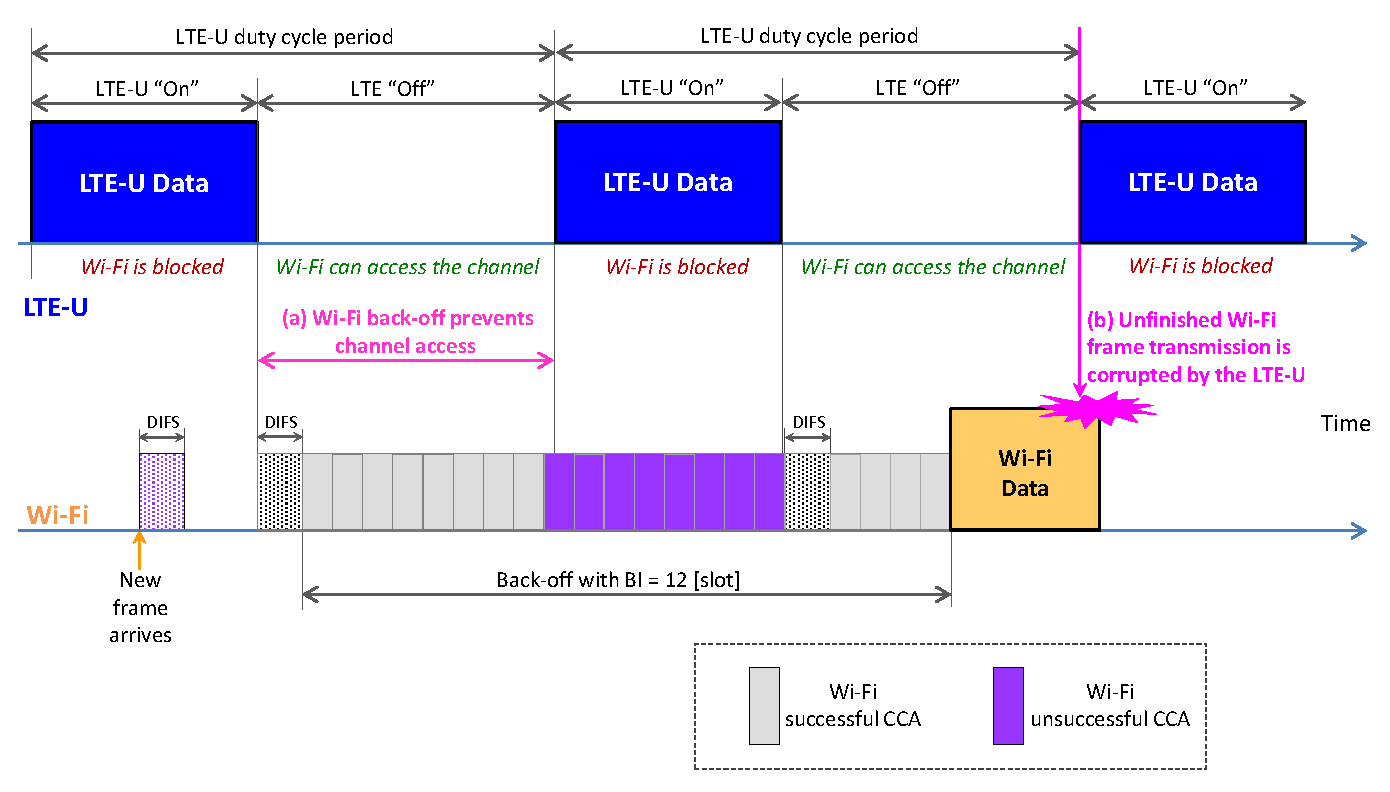
\includegraphics[width=1.0\columnwidth]{figures2/LTE-U-enhancement1}
\caption{Negative interactions between LTE-U and Wi-Fi systems.}
\label{figs:LTE-U-enhancement1}
\end{figure}

\subsection{LTE-U-aware CSMA-CA and LTE-U with LBT}
\label{subsection:LTE-U-aware}

LTE-U mostly assumes neither coordination nor synchronization between itself and Wi-Fi system. LTE-U's ``on'' and ``off'' cycles are only known by LTE devices themselves. Vice versa, Wi-Fi control and management frames are known by Wi-Fi devices themselves. This independent operation results in various transmission issues. \textit{First}, in cases when LTE-U's ``on'' duration is not sufficiently long while Wi-Fi exponential back-off procedure generates long back-off intervals, Wi-Fi STAs may not have a chance to utilize the channel when LTE-U is not active. Such a conservative channel access principle wastes the radio resources and results in Wi-Fi's poor performance. \textit{Second}, an unfinished Wi-Fi frame transmission that was started during the LTE-U's ``off'' duration might be corrupted by the LTE frames once LTE switches to ``on'' cycle. Fig. \ref{figs:LTE-U-enhancement1} visualizes two examples.

To mitigate these issues, inter-RAT communications between LTE and Wi-Fi could be employed to inform Wi-Fi system the LTE-U's ``on'' and ``off'' cycles. Wi-Fi system then can adapt its MAC protocol (i) to occupy the channel more opportunistically during LTE-U's ``off'' period (but not to increase the collision probability among Wi-Fi STAs) and (ii) to schedule frame transmissions in such a way that they will not step on the next LTE-U's ``on'' cycle. Besides, frame collisions could be mitigated by incorporating some form of LBT/CCA into LTE-U. Specifically, CCA should be performed before activating LTE-U's ``on'' cycle. If the channel is detected busy, LTE-U's ``on'' cycle is deferred.

\begin{figure}[!t]
\centering
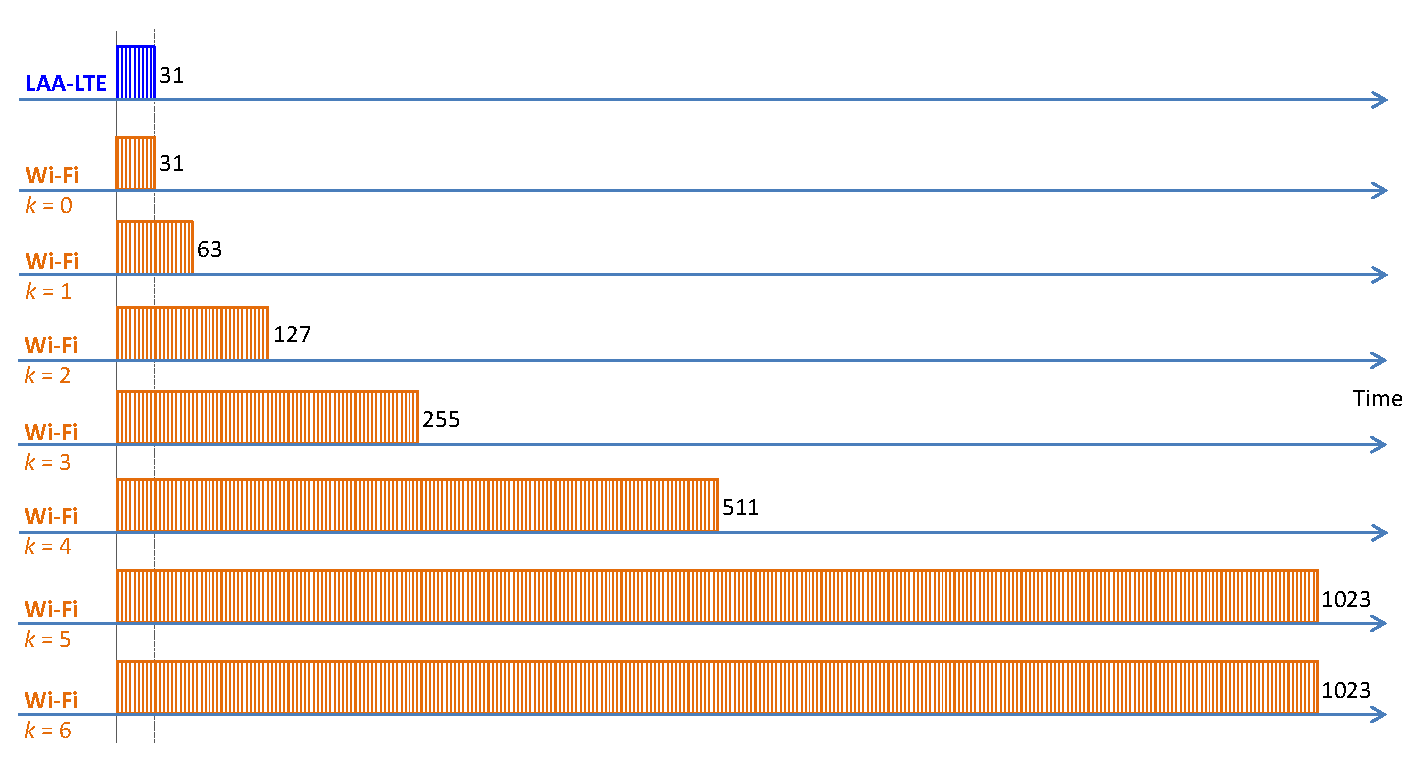
\includegraphics[width=1.0\columnwidth]{figures2/LAA-LTE-enhacement-back-off}
\caption{Wi-Fi exponential back-off competes for the channel more conservatively, compared to LAA-LTE.}
\label{figs:LAA-LTE-enhacement-back-off}
\end{figure}

\subsection{LAA-LTE with Exponential Back-off}
\label{subsection:exp-back-off}

While LBT, as a general approach, can be a good basis for coexistence of LAA-LTE and Wi-Fi, the LBE LBT in its current form (as introduced by European regulations) which is adopted for LAA-LTE is still unfair to Wi-Fi. LAA-LTE nodes impact Wi-Fi nodes in terms collision rate and probability of successful channel access more than similar Wi-Fi nodes on the same carrier. This is not compliant with the objectives as listed in 3GPP LAA LTE Study Item \cite{LAA-LTE-SI}: ``LAA should not impact Wi-Fi services (data, video and voice services) more than an additional Wi-Fi network on the same carrier; these metrics could include throughput, latency, jitter, etc.''. One major and obvious reason is, that while Wi-Fi applies exponential back-off rule, LAA-LTE simply applies fixed-size back-off rule. In order to elaborate this observation, consider a typical example follows. It is assumed that $W^{\mathrm{LAA-LTE}}=31$, $W^{Wi-Fi}_{\min}=31$, and $W^{\mathrm{Wi-Fi}}_{\max}=1023$. Then, as descirbed in subsection \ref{subsection:LAA-LTE}, LTE-U always back-offs with contention window $W^{\mathrm{LAA-LTE}}=31$. For Wi-Fi, as descirbed in subsection \ref{subsubsection:IEEE 802.11 CSMA-CA}, it back-offs with contention window $W(0)=31$ for the initial transmission attempt. However, if collisions occur, it progressibly doubles its contention windows to reduce the probability of a subsequent collision: $W(1)=63$ (the first re-transmission attempt), $W(2)=127$ (the second re-transmission attempt), $W(3)=255$ (the third re-transmission attempt), $W(4)=511$, $W(5)=1023$, $W(6)=1023$, and etc. Fig. \ref{figs:LAA-LTE-enhacement-back-off} compares contention windows of LAA-LTE and Wi-Fi.

At present, there is no existing work that studies how an exponential back-off can help to improve the fairness between LAA-LTE and Wi-Fi. It is important to note that, compared to Wi-Fi, designing an exponential back-off protocol for LAA-LTE that employs OFDMA-based MAC layer might not be straightforward. In details, Wi-Fi adopts OFDM in the PHY layer and allows only one user to occupy the whole channel at one time. Its contention window is scaled respectively to the outcome (success or failure) of a frame transmission to given user. For LTE, OFDMA devides the system bandwidth into a series of Physical Resource Blocks (PRBs). Each PRB is composed of $12$ OFDM subcarriers. Different PRBs can be allocated to different users in a given subframe and multiple users can occupy the channel at the same time. This implies that the rule governing the adaptation of contention window of LAA-LTE is required to be more sophisticated than that of Wi-Fi. In adddition to back-off procedure design, there are two other interesting questions: (i) how exponential back-off could (negatively) affect the performance and efficiency of LAA-LTE; and (ii) what could be appropriate values for LAA-LTE's operation parameters.

A side note is that, according to \cite{U-LTE-FCC-Cisco-2015}, 3GPP is now having a working agreement to use a LBT mechanism with exponential back-off. At this moment, LAA-LTE standard is not yet finalized by 3GPP and no information is publicly available. ETSI is also devising a set of minimum ``fairness'' requirements as part of EN 301 893 standard for ``5 GHz high performance wireless access systems'' in Europe (scheduled to be completed by the end of 2015).

\begin{figure}[!t]
\centering
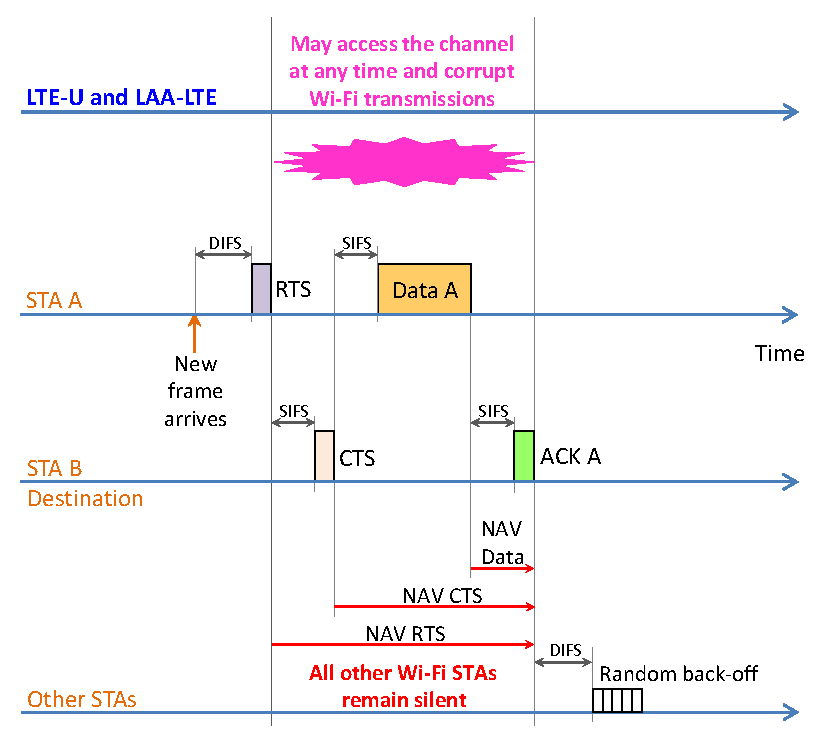
\includegraphics[width=0.7\columnwidth]{figures2/LTE-U-enhancement-RTS-CTS-NAV}
\caption{U-LTE may cause channel collisions with Wi-Fi at any time.}
\label{figs:LTE-U-enhancement-RTS-CTS-NAV}
\end{figure}

\subsection{Wi-Fi-aware LTE-U and LAA-LTE}
\label{subsection:Wi-Fi-aware}

As addressed in subsection \ref{subsubsection:IEEE 802.11 CSMA-CA}, RTS/CTS and NAV are effective and important mechanisms employed by the IEEE 802.11 CSMA-CA protocol to reserve the channel and avoid collisions. However, since U-LTE and Wi-Fi are not collaborating, Wi-Fi's NAV information carried by RTS, CTS, and data frames is not known by U-LTE devices. In other words, while Wi-Fi STAs defer their transmissions until ongoing frame exchanges are done, U-LTE devices do not respect Wi-Fi reservation and may start their transmissions at any time, as shown in Fig. \ref{figs:LTE-U-enhancement-RTS-CTS-NAV}. This may result in a high rate of channel collisions and corrupt both Wi-Fi and U-LTE transmissions. As visualized Fig. \ref{figs:LTE-U-enhancement-RTS-CTS-NAV}, an U-LTE transmission could accidentally destroy the whole Wi-Fi transmission session composing of RTS, CTS, data, and ACK frames (at the same time, U-LTE frame is also corrupted by Wi-Fi frames). Mechanisms that provide U-LTE with information on Wi-Fi activities to avoid such transmission corruptions could be therefore very beneficial.

\subsection{Collaborative U-LTE and Wi-FiCollaborative U-LTE and Wi-Fi}

As metioned so far, almost all existing works dealing with U-LTE and Wi-Fi coexistence assume non-cooperative approach which does not required any information exchange between these two networks. LTE is simply additionally equipped with some mechanisms to friendly share the same channel with existing Wi-Fi networks. The authors in \cite{U-LTE-5G-2015, Coordinated-LTE-U-Wi-Fi-2015} carry out preliminiary investigations towards this direction. However, only conceptual network archirectures and mechanisms and are presented. Collaborative approaches is quite interesting since it may result in better coexistence by sharing information between different radio access technologies (RATs) and enabling global/local optimizations. Some benefits of such approaches has been outlined in subsections \ref{subsection:LTE-U-aware} and \ref{subsection:Wi-Fi-aware}. This approach, on the other hand, may be challenging since it needs additional network infrastructure/entities and set of protocols for inter-RAT communications. They are required for discovery of neighboring radio systems, selecting operating channels/transmission power, etc., for radio systems, and providing some level of fair and/or efficient use of available channels. 


\subsection{Inter-operator U-LTE Coexistence}

In addition to coexistence between U-LTE and Wi-Fi, coexistence among U-LTE systems deployed by different operators running in a shared band is also a critical concern. This concern is more pronounced in high density urban areas with a very large number of devices/system running different protocols. Work in \cite{LTE-U-ICC-WS-2015} presents a preliminary study on this and the results show that LBT mechanisms can increase the network throughput since collisions can be mitigated. Work in \cite{Enhanced-LTE-U-thesis-2015} investigates the interactions between different LBT mechanisms when they are deployed in proximity of each other. Inter-operator U-LTE coexistence is especially important when multiple operators employ similar MAC protocols based on fixed contention windows that could be accidentally synchronized in channel access attemps and result in consecutive collisions. As a result, exponential back-off rules, inter-RAT communications, and collaborative inteference management protocols could be promising approaches.

\subsection{Other Considerations on Coexistence}

Operations, system performance, and coexistence of radio networks highly depend on deployment scenarios. This is the main reason why a number of existing work supports U-LTE technology while the others call for further investigations and developments before deploying this technology. Also, different coexistence mechanisms are recommended for different scenarios. For a complete understanding of U-LTE impacts on Wi-Fi, a wide range of node and load densities should be considered. Besides, performance of voice and video-related applications should be evaluated. For most of existing work, only throughput and channel access probability of Wi-Fi networks are evaluated. However, an insight to latency and jitter performance could be desirable. Besides, it would be interesting to take into account the operations and performance of recent Wi-Fi variants when coexisting with U-LTE.

\subsection{Emerging Wi-Fi Technologies and U-LTE}

With the currrent trends of future RANs including network densification, heterogeneous network (HetNet), Internet of Things (IoT), the explosion of various applications (smart homes/cities, smart transportations, automomous vehicles, etc.), and etc., numberous technological evolutions have been expecting. For time-sensitive applications (e.g., sensor and control for critical infrastructures and automomous vehicles), data communications is required to be extremely reliable, robust, energy-efficient while being able to guaratee latencies in millisecond or sub-millisecond scale. These requirements urge for the developments of collaborative, well-controlled, and synchronous Wi-Fi MAC protocols (instead of distributed, random-access-based, and asynchronous IEEE 802.11 CSMA/CA that have been widely deployed). To this end, PCF and HCCA operation schemes (specified in IEEE 802.11/802.11e standards but not widely used) should be re-visited.

Despite the fact that PCF and HCCA allocate the channel to STAs in a well-controlled manner, their performance (in terms of throughput, latency, and power consumption) is still questionable due to their complexities and signaling overheads, specially in highly dense networks with a vast number of battery-operated devices exchanging short and bursty messages. Furthermore, it is compelling to understand their interaction and coexistence with U-LTE. While CFP and CAP are desired for time-sensitive applications, the aggressive operation of U-LTE in the same frequency band may render them impossible. Finally, protocols and enabling technologies for collaborations and synchronizations between PCF-/HCCA-based Wi-Fi and U-LTE appear to be essential and thus could be very interesting working areas.

\subsection{Further Investigation on MuLTEfire}

At this time there are very few technical details available about MuLTEfire. It is unknown which MAC protocols or coexistence mechanisms are employed in this type of U-LTE. Also, since licensed frequency is not used for LTE network management and control signaling, as opposed to the conventional LTE and the other two variants of U-LTE (i.e., LTE-U and LAA-LTE) that are license anchored, MuLTEfire may lose all advantages of native LTE technologies. It is expected that MuLTEfire will be less efficient than LTE-U and LAA-LTE and therefore its achievable performance/efficiency may be just marginally better than that of Wi-Fi. Then the question on the applicability of MuLTEfire needs to be answered.


%**************************************************************************************************************%
\section{Conclusions}
\label{sec:conclusions}

\noindent This work ...



%**************************************************************************************************************%
\section*{Acknowledgment}

{\small
\noindent This work was partially supported by the Natural Sciences and Engineering Research Council (NSERC) through the NSERC Strategic Network for Smart Applications on Virtual Infrastructure (SAVI), and the Fonds Qu\'{e}b\'{e}cois de la recherche sur la nature et les technologies (FQRNT) via a scholarship.
}


%**************************************************************************************************************%
\bibliographystyle{IEEEtran}
\bibliography{U-LTE}


\vfill{}

\end{document}
